

\chapter{Material and methods}

%  Everything that is mentioned in results, has to be mentioned here
%  Everybody who reads thesis, must be able to reproduce the experiment/study
% o Describe all materials, devices and methods, which were used in your work
% o if you describe a device, start with the brand name followed by the company name, city and country in parentheses: e.g. "... a VersaHD (Elekta AB, Stockholm, Sweden) was used in ...".
% o Provide some information on each device
%  e.g Linac, which energies were used, what was the field size, what was the leaf width, how is the linac calibrated, ...;
%  e.g. Detector array: which type of detector, how many detectors, what is the resolution, energy dependence, linearity,...;
%  e.g. Panning systems: software version, algorithms, settings used in this study
%  e.g. software: version, functionality
% o Also describe used data (patient cohort) even if they were taken from other studies

\section{Scanners and imaging protocols}

For this thesis a CT scanner and an open-bore, c-arm MR scanner in the radiation oncology department of the Vienna General Hospital (AKH) were used.

\subsection{MR}

Following the general practice of phantom measurements, and the AAPM recommendations on phantom filling materials [AAPM 1990 and 2010]/ \cite{Jackson2009} oils or water with addition of paramagnetic substances (to reduce the spin-lattice relaxations times) were chosen (generally short T1 time of ~200-400 ms).
This, combined with a T1-weighted test sequence, improves the efficiency of the measurements assuring relatively high SNR in short time.
To further improve image quality, the averaging parameter of the test sequence was set to 4.
This setting practically means the measurement is repeated and averaged $n$ times by the scanners software.
Remaining sequence parameters were optimized to yield an acceptable resolution for the chosen ROI setting (which is relatively large as it covers the whole phantom).
The test sequence was chosen in a way, such as to deviate as little as possible from a typically used clinical imaging setting.
However, to fully understand and investigate the possible image distortions, each clinically used sequence should be commissioned with a distortion phantom.
Detailed sequence parameters are listed in table \ref{tab:MR-scanner}


\begin{table}[!tbh]
\centering
\caption{MR scanner and used protocol.}
\begin{tabular}{r|l}
system			& MRI				\\
\toprule
manufacturer	& Siemens			\\
product name	& Magnetom C!		\\
coil [internal W x H]	& Body/Spine Array Coil XL [$50\, $x$ \,30.5\, cm$ ($19.7\, $x$ \,12\, $in)]	\\
orientation		& axial	\\
sequence		& T1 weighted 3D-FLASH Vibe	\\
				& (Volumetric interpolated breath-hold)	\\
slice thickness	& $2.3\, mm$	\\
pixel spacing	& $2.3\, mm$	\\
matrix			& 128 x 120 \\
repetition time & $7.07\, ms$	\\
echo time		& $2.7\, ms$	\\
bandwidth		& 240	\\
flip angle		& $6\, deg$	\\
averages $n$	& 4	\\
acquisition time& $17.5\, min$
\end{tabular}
\label{tab:MR-scanner}
\end{table}


\subsection{CT}
To generate a reference CT image set a typically used clinical pelvis imaging protocol for radiation therapy planning (with increased resolution 0.6 mm) was used (see table \ref{tab:CT-scanner}).

\begin{table}[!tbh]
\centering
\caption{CT scanner and used protocol.}
\begin{tabular}{r|l}
system			& CT				\\
\toprule
manufacturer	& Siemens			\\
product name	& SOMATOM Definition AS		\\
software version& syngo CT 2013B	\\
protocol		& Prostatae\_VMATAdult	\\
slice thickness	& $0.6\, mm$	\\
row spacing		& $0.801\, mm$; 512	\\
column spacing	& $0.801\, mm$; 512	\\
kVP				& $120\, kV$	\\
x-ray tube current	&	$19\, mA$	\\
convolution kernel	&	I30f, 3
\end{tabular}
\label{tab:CT-scanner}
\end{table}


\subsection{MR scanner - field distribution}
\label{sec:magnetom}

Diagrams of the magnetic field strength are depicted in figure \ref{fig:strength_side}); its gradient in figures \ref{fig:gradient_side}, \ref{fig:gradient_top} and \ref{fig:gradient_front}).
Figure \ref{fig:scanner} shows an image and different views of the scanner and the planes along which the field strength and gradient are displayed.
For imaging, the patient is positioned as to place the ROI at the isocentre, the area where the $B_0$ field is most homogeneous (where there is a low gradient).

\begin{figure}[!htb]
\centering
  \begin{subfigure}[b]{0.4\textwidth}
	\centering
	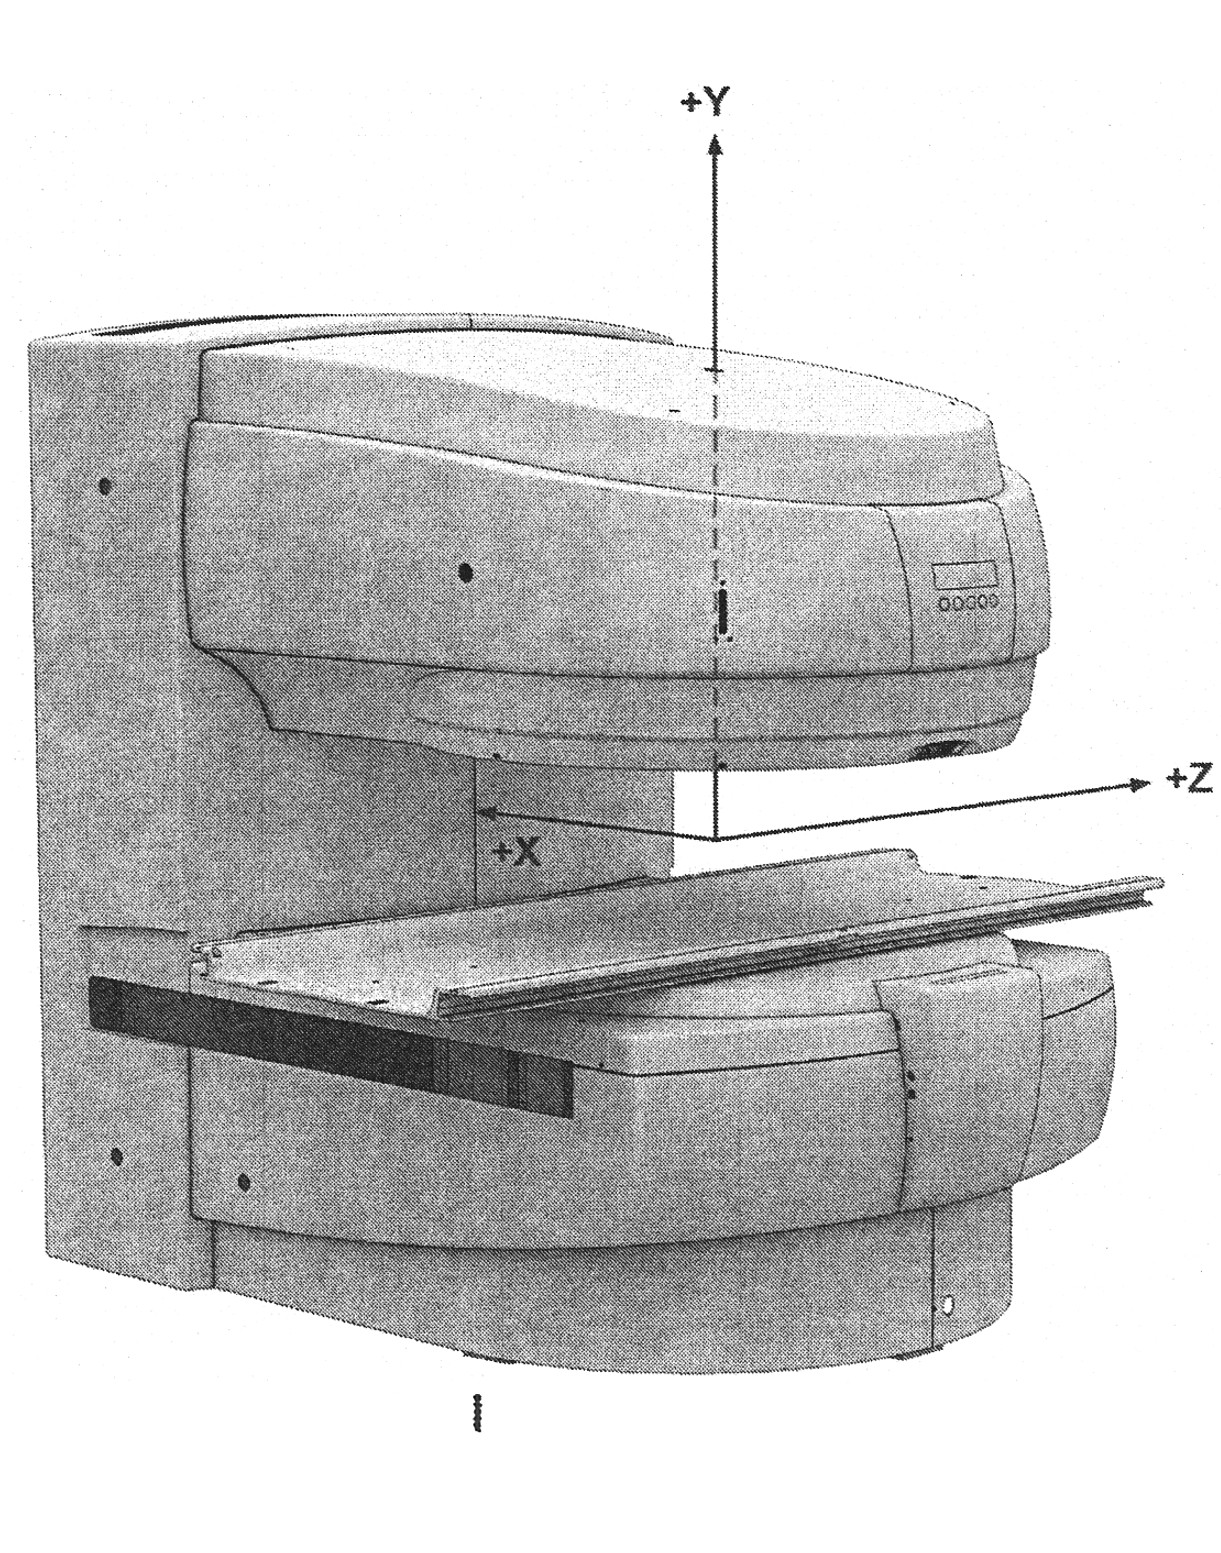
\includegraphics[scale=0.7]{scanner/scanner_img.jpg}
	\caption{Image of scanner\\ x,y, \& z -axis}
	\label{fig:scanner_image}
  \end{subfigure}
    \hfill
  \begin{subfigure}[b]{0.4\textwidth}
  	\centering
    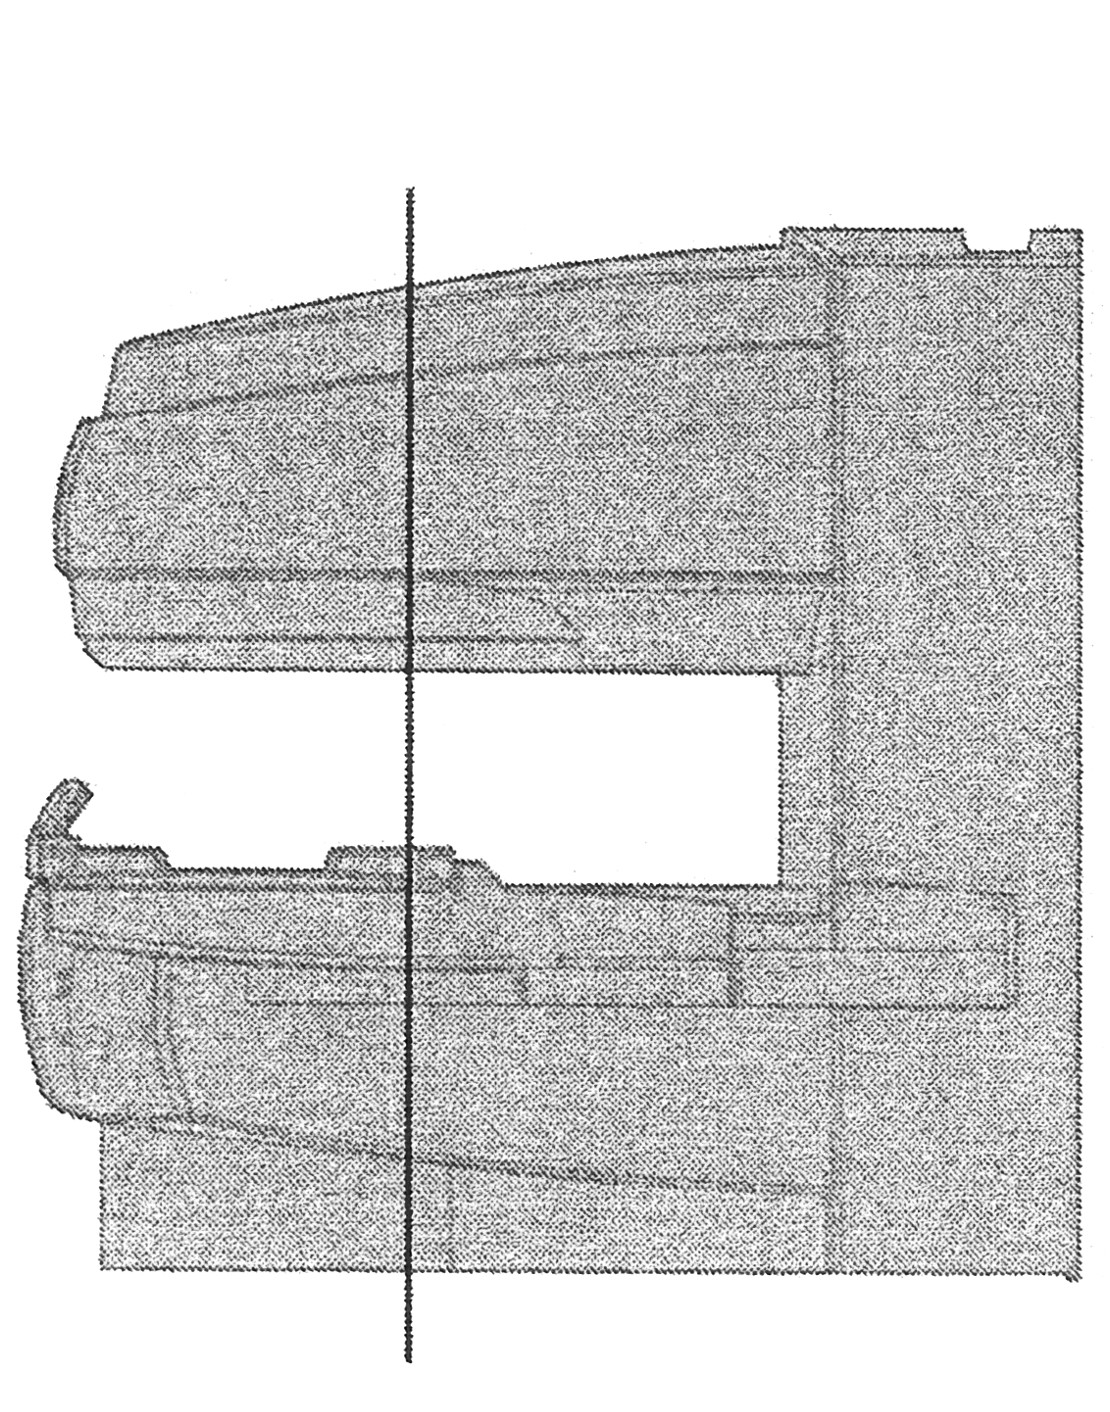
\includegraphics[scale=0.7]{scanner/scanner_front.jpg}
    \caption{side view along z-axis,\\ black line represents plane for front view (see fig. \ref{fig:gradient_front})}
    \label{fig:scanner_front}
  \end{subfigure}
  
  \begin{subfigure}[b]{0.4\textwidth}
   	\centering
   	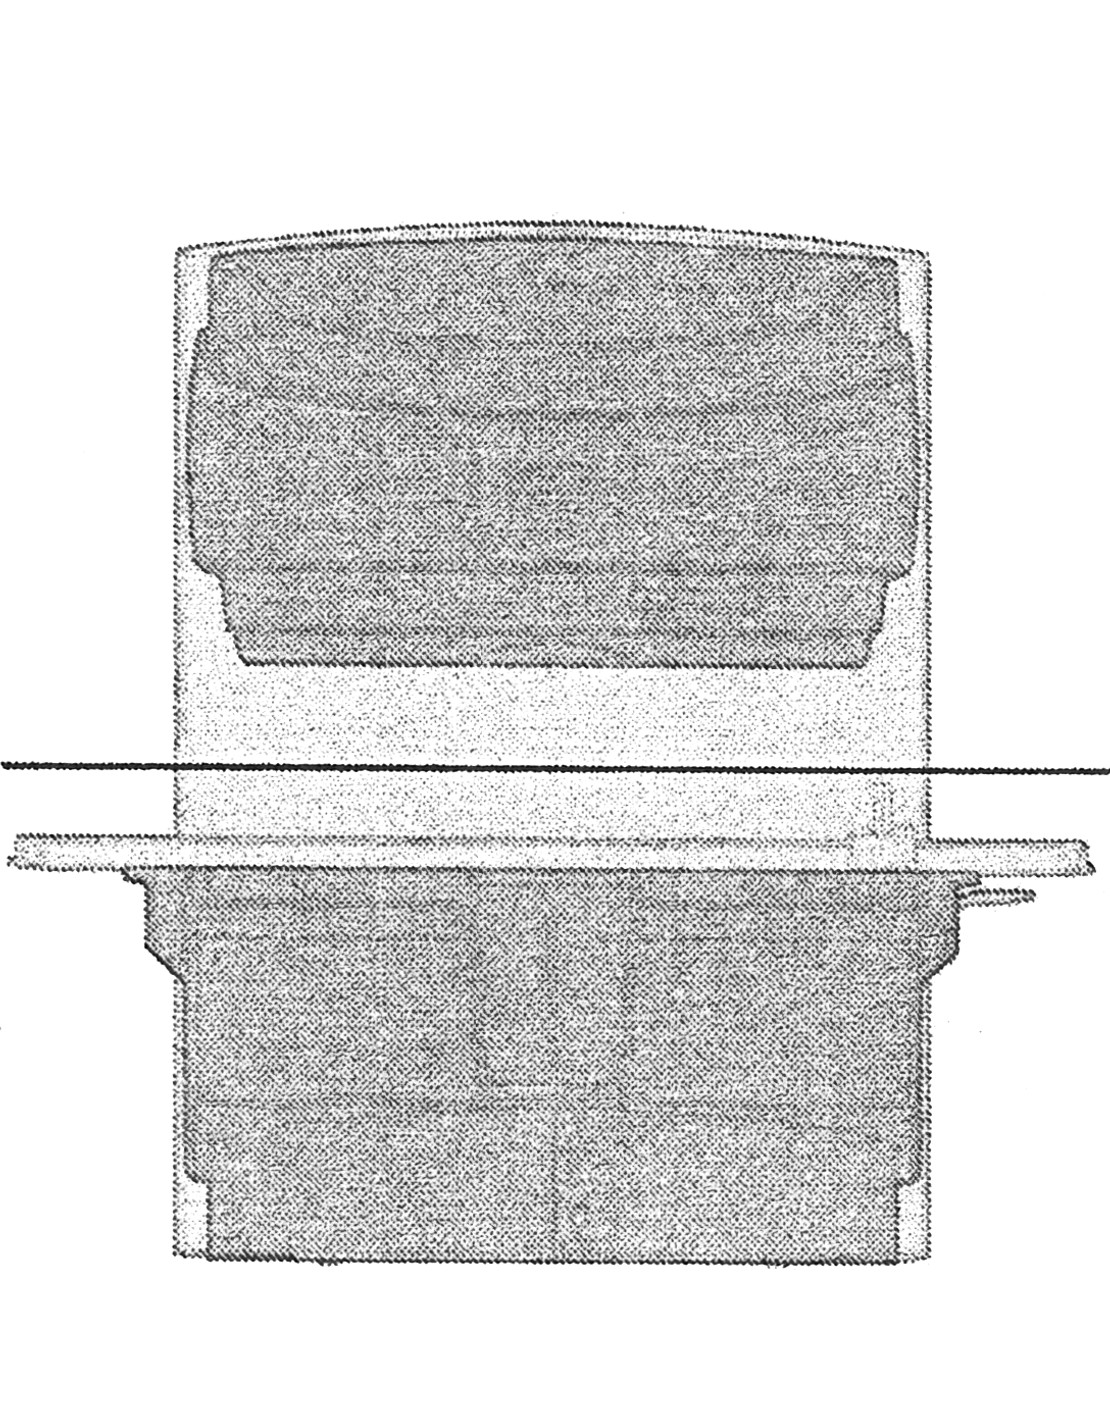
\includegraphics[scale=0.7]{scanner/scanner_top.jpg}
   	\caption{front view along x-axis,\\ black line represents plane for top view (see fig. \ref{fig:gradient_top})}
   	\label{fig:scanner_top}
  \end{subfigure}
    \hfill
  \begin{subfigure}[b]{0.4\textwidth}
  	\centering
  	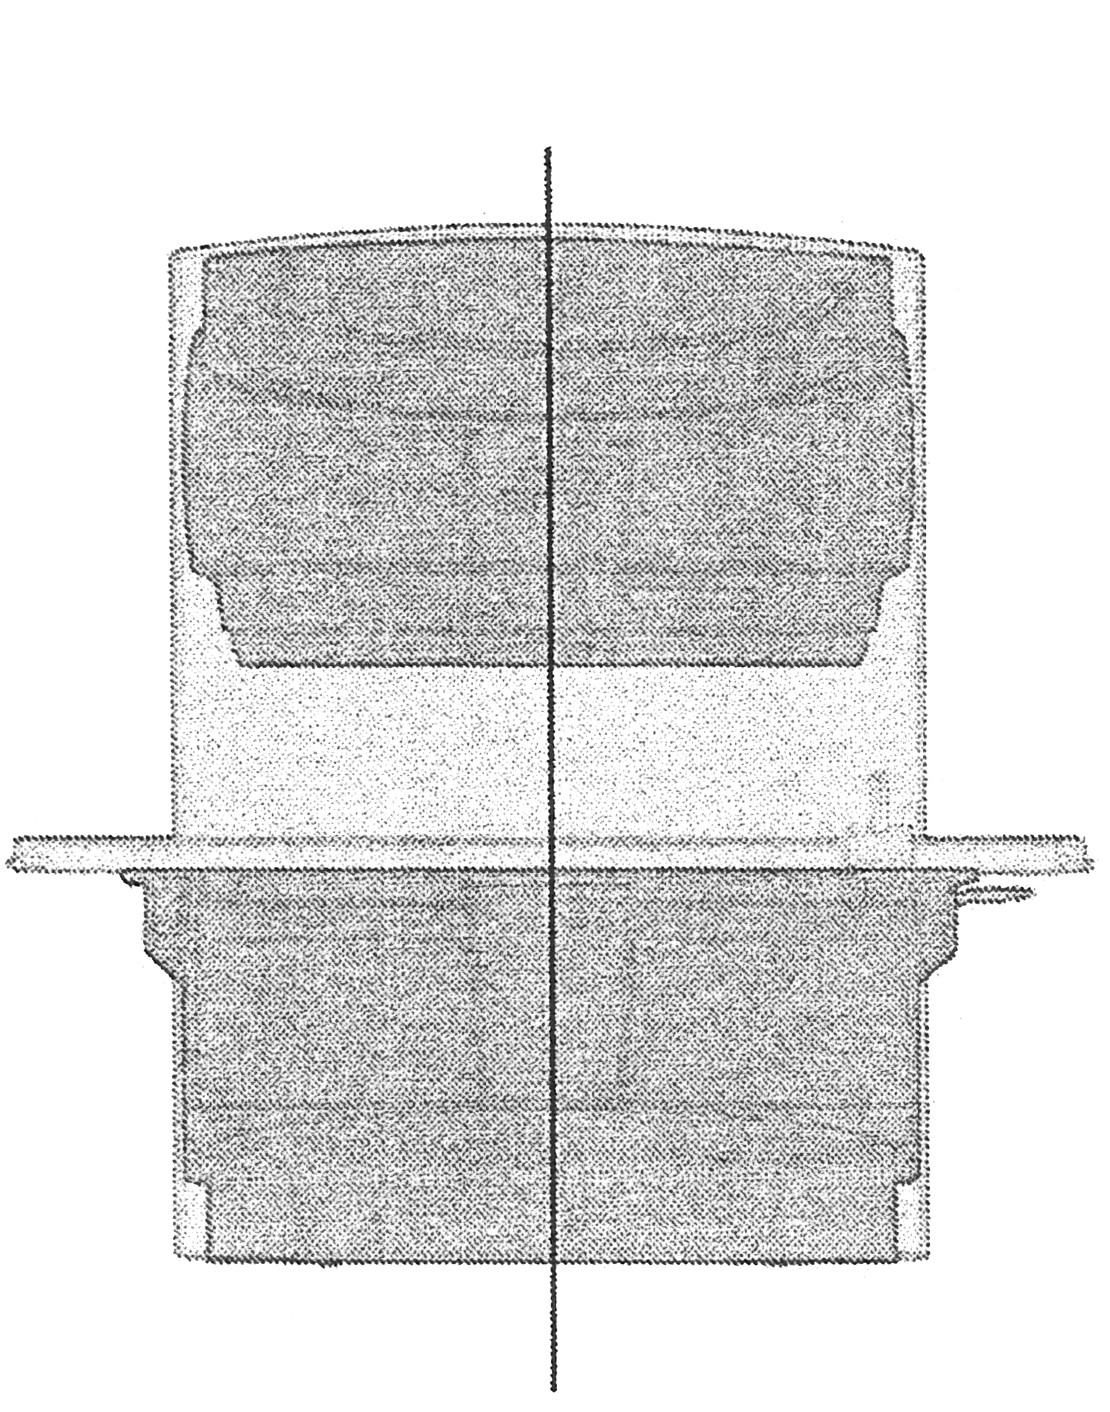
\includegraphics[scale=0.7]{scanner/scanner_side.jpg}
  	\caption{front view along x-axis,\\ black line represents plane for side view (see fig. \ref{fig:gradient_side} and \ref{fig:strength_side})}
  	\label{fig:scanner_side}
  \end{subfigure}
  \caption[Magnetom C! Image source: \cite{magnetom_handbook}]{Magnetom C! Image source: \cite{magnetom_handbook} (with kind support of Siemens Healthineers)}
  \label{fig:scanner}
\end{figure}

%diagrams as individual figures:
\begin{figure}[!htb]
  	\centering
      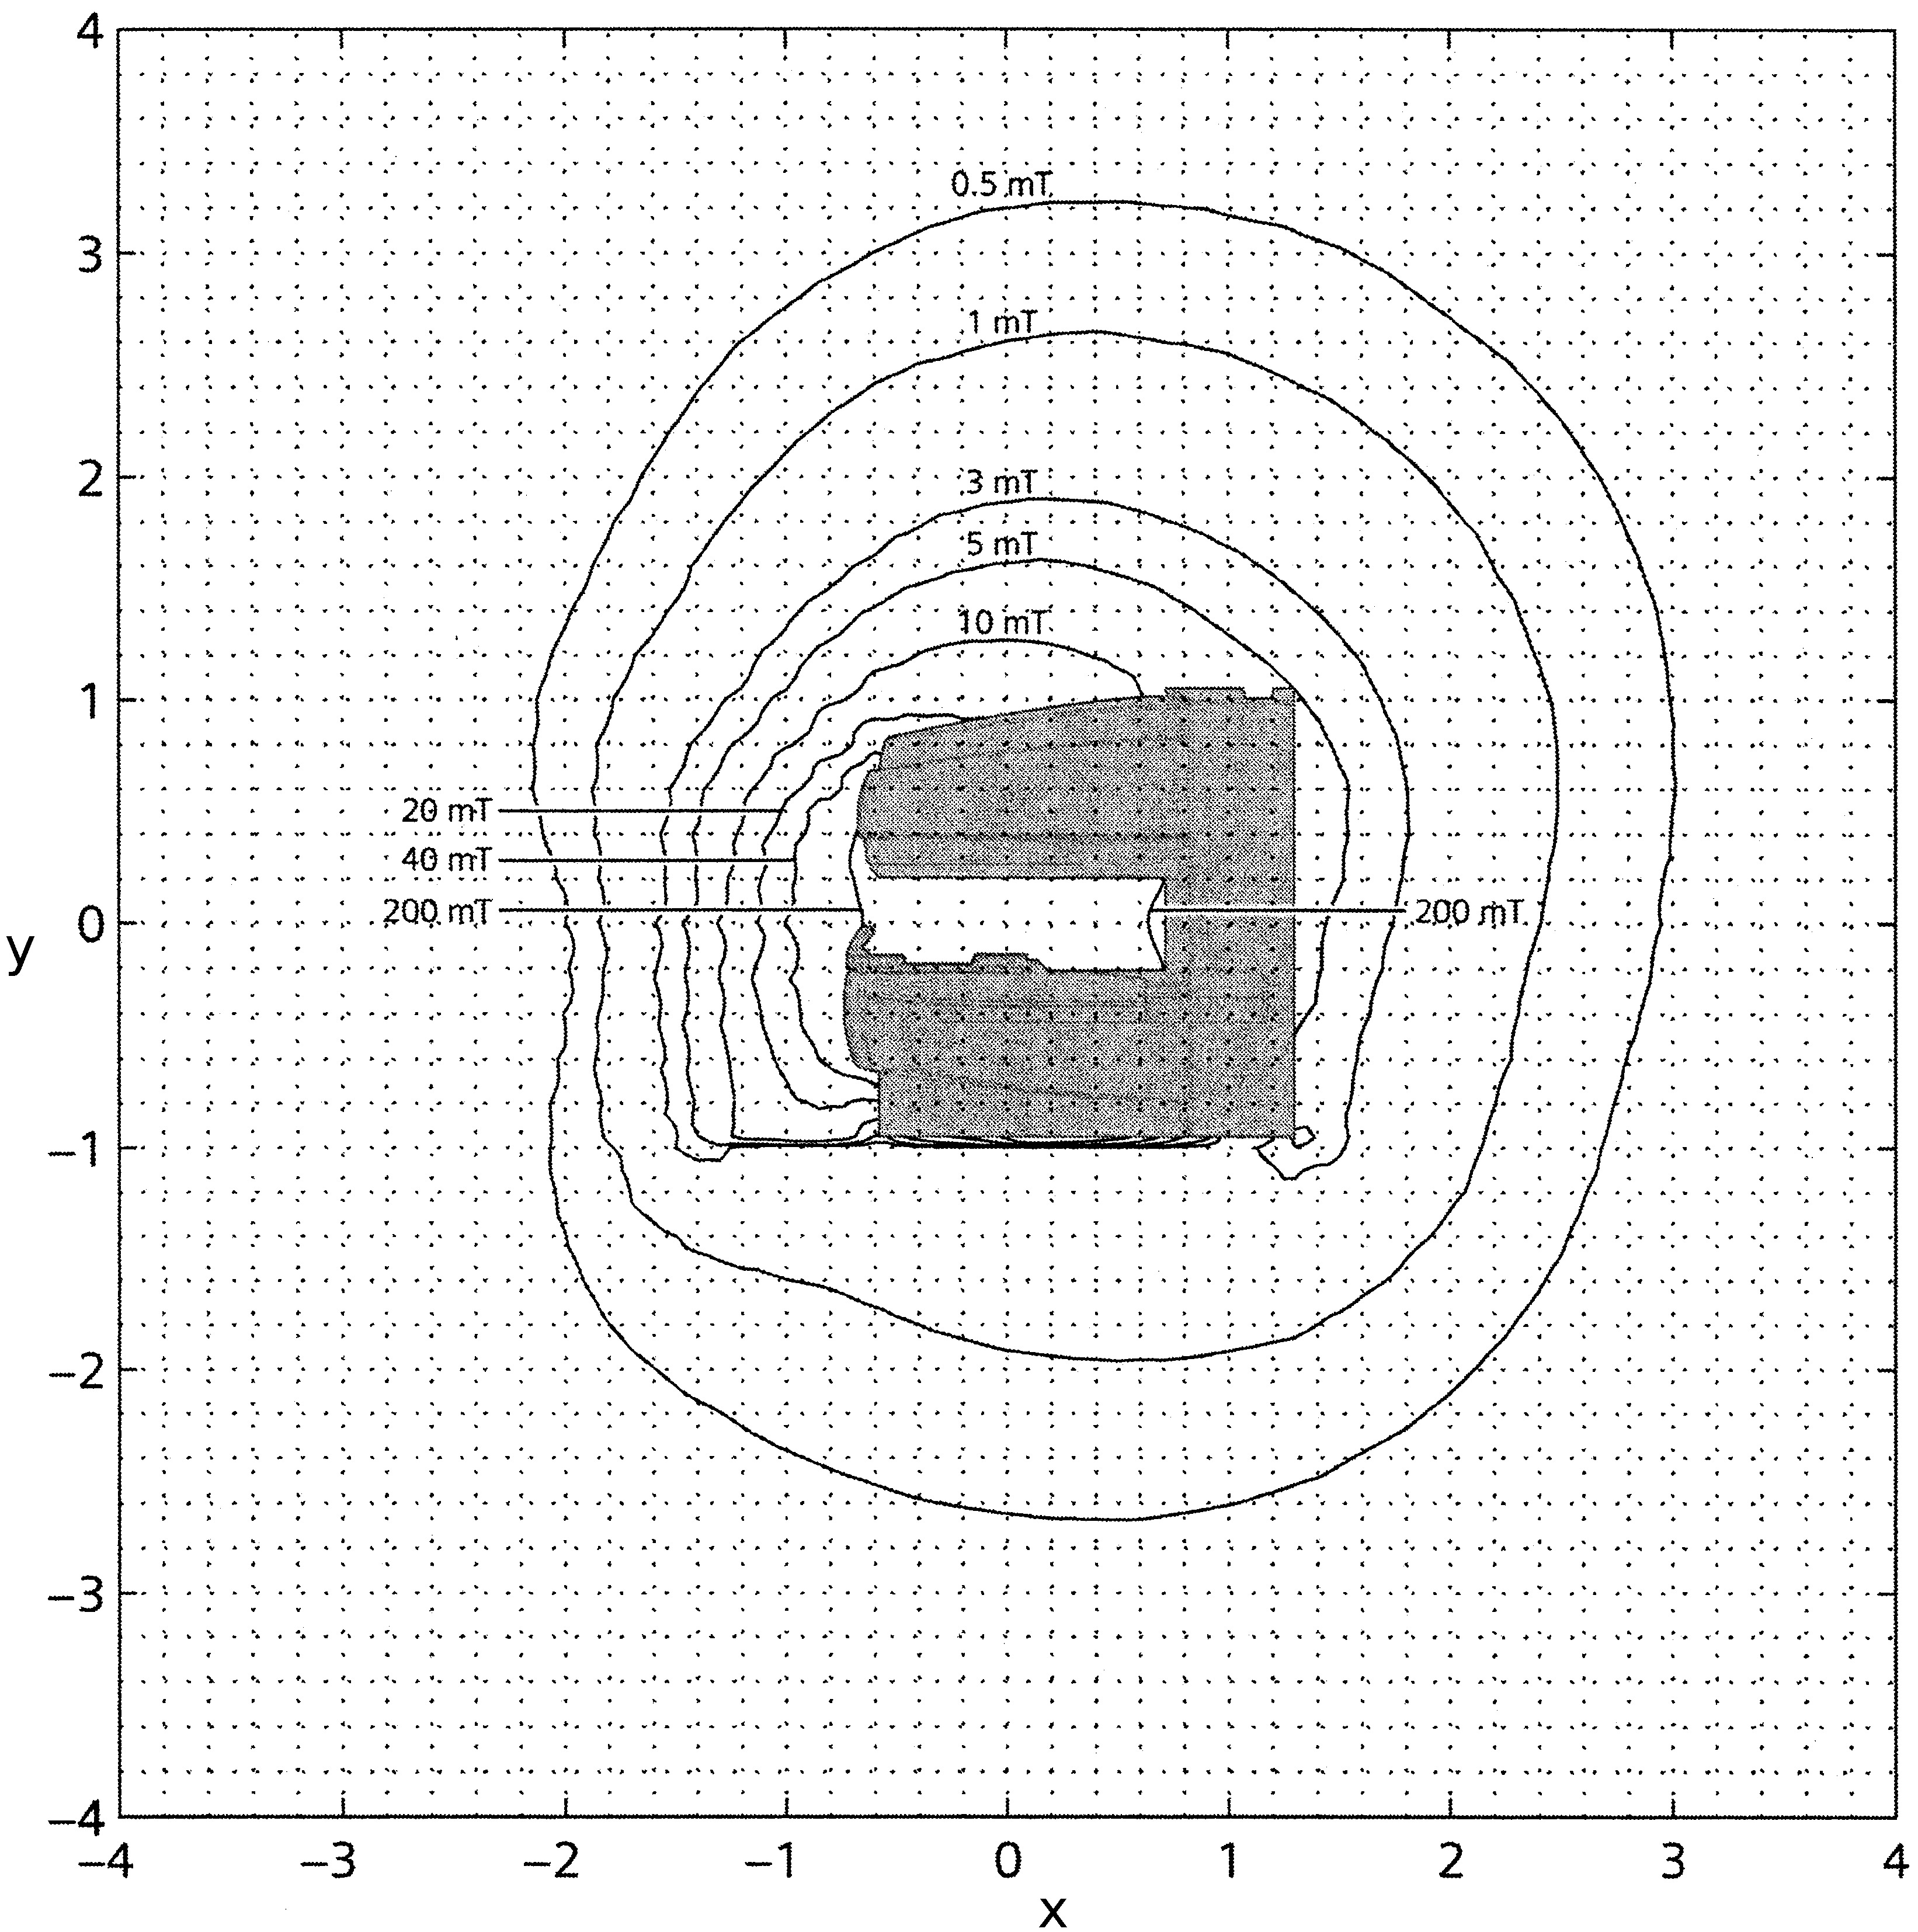
\includegraphics[scale=1.1]{scanner/scanner_field-strength.jpg}
      \caption[Magnetom C! field strength\\ side view along z-axis. Image source: \cite{magnetom_handbook}]{Magnetom C! field strength\\ side view along z-axis (see fig. \ref{fig:scanner_side}). Image source: \cite{magnetom_handbook} (with kind support of Siemens Healthineers)}
    \label{fig:strength_side}
\end{figure}

\begin{figure}[!htb]
    	\centering
        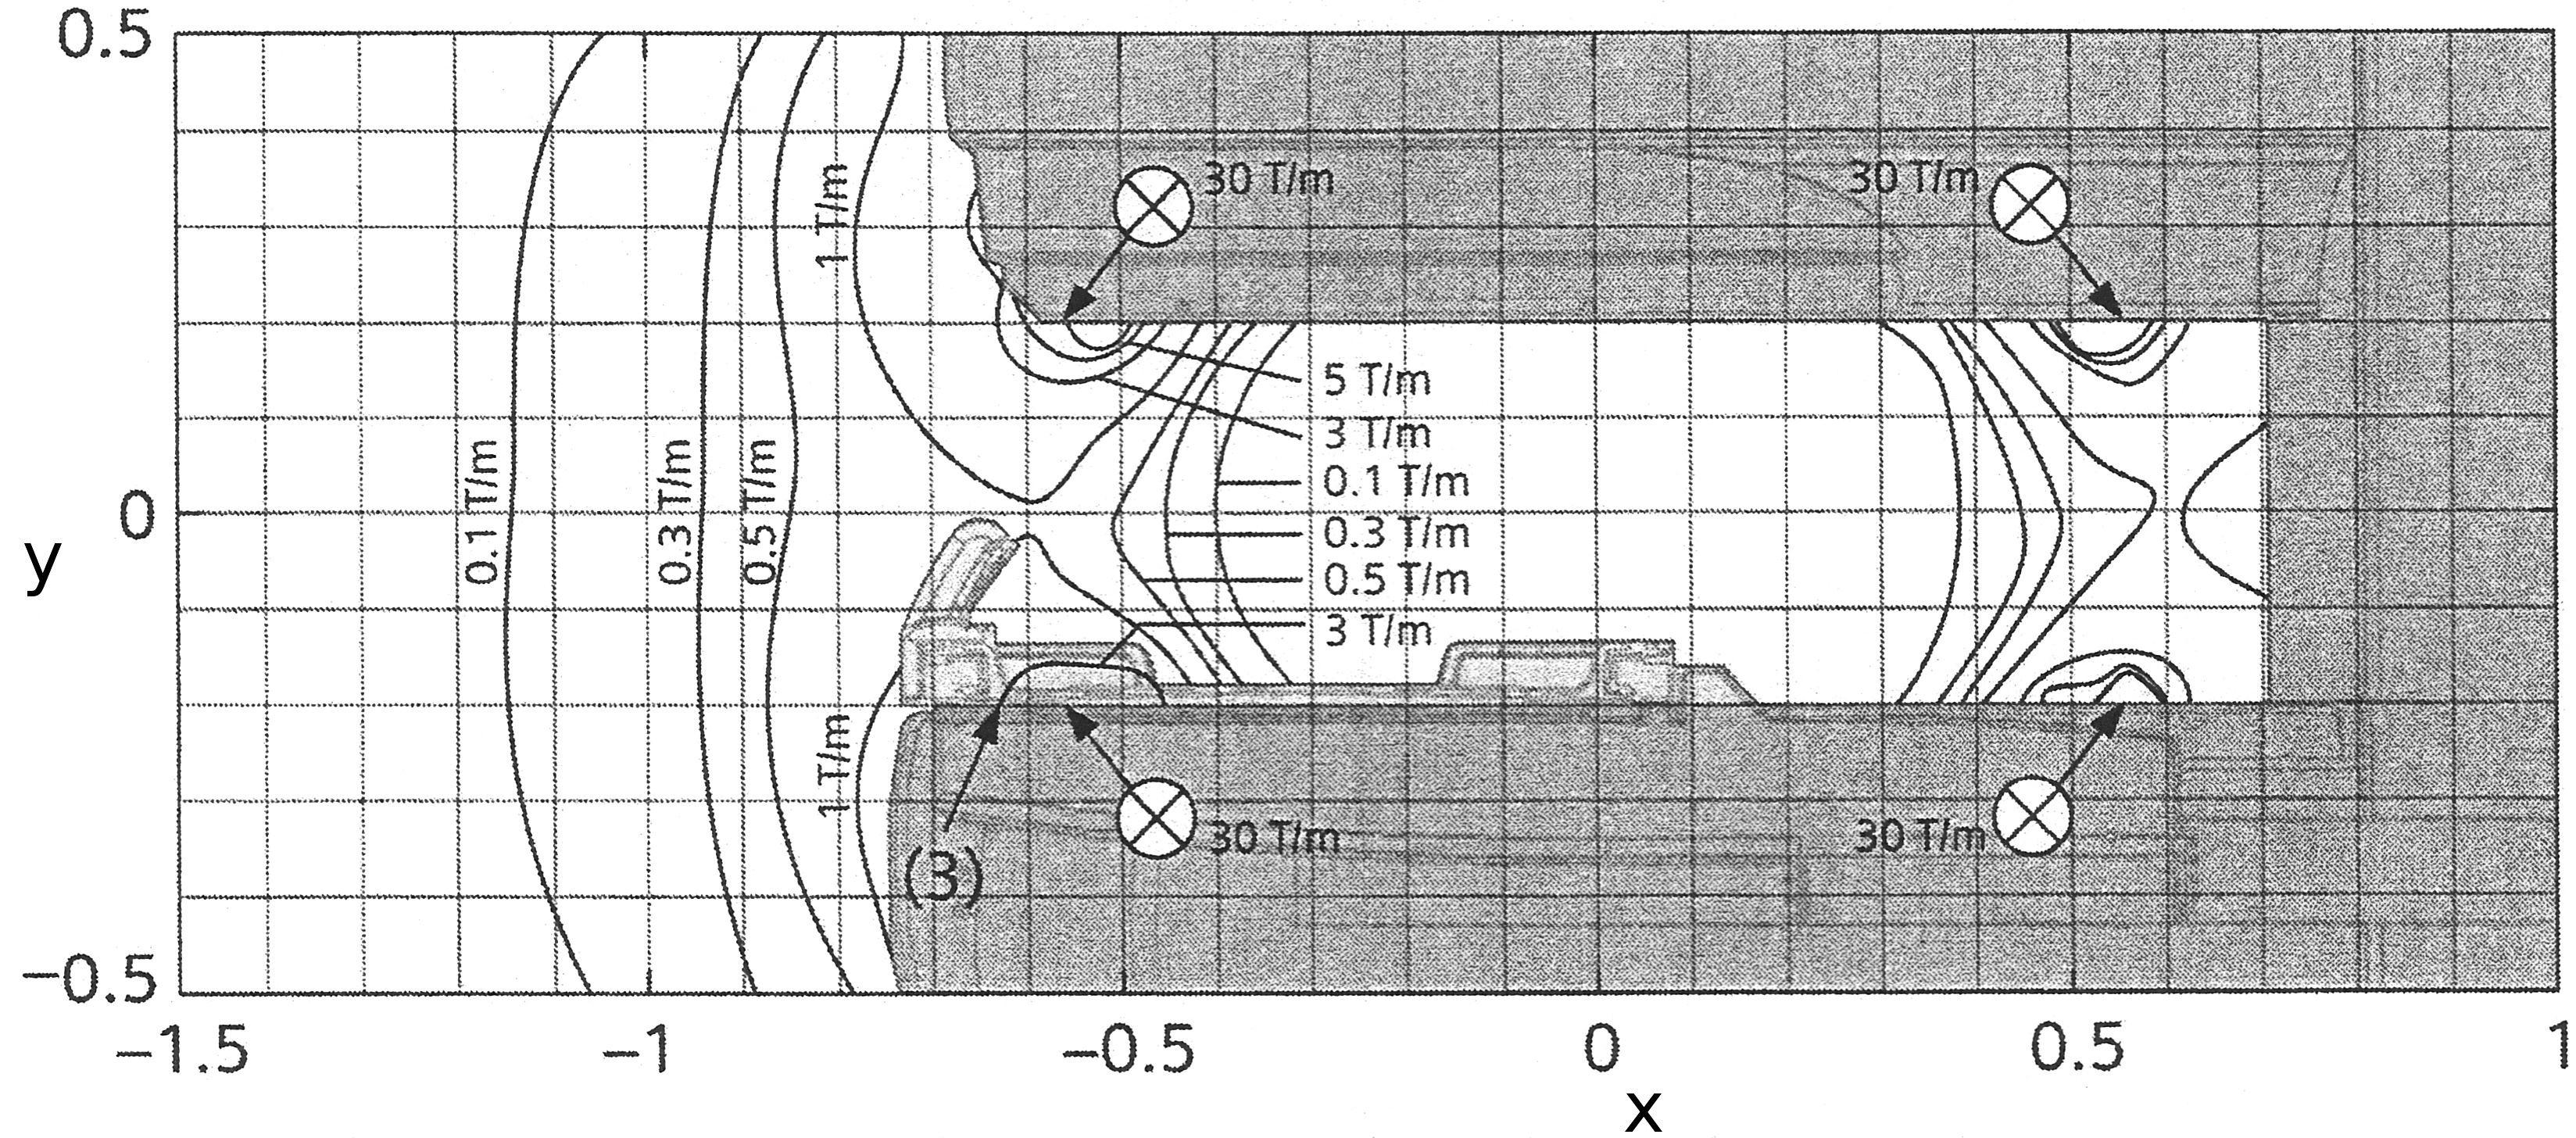
\includegraphics[scale=1.1]{scanner/scanner_gradient-side.jpg}
        \caption[Magnetom C! field gradient\\ side view along z-axis. Image source: \cite{magnetom_handbook}]]{Magnetom C! field gradient\\ side view along z-axis (see fig. \ref{fig:scanner_side}). Image source: \cite{magnetom_handbook} (with kind support of Siemens Healthineers)}
        \label{fig:gradient_side}
\end{figure}

\begin{figure}[!htb]
  	\centering
    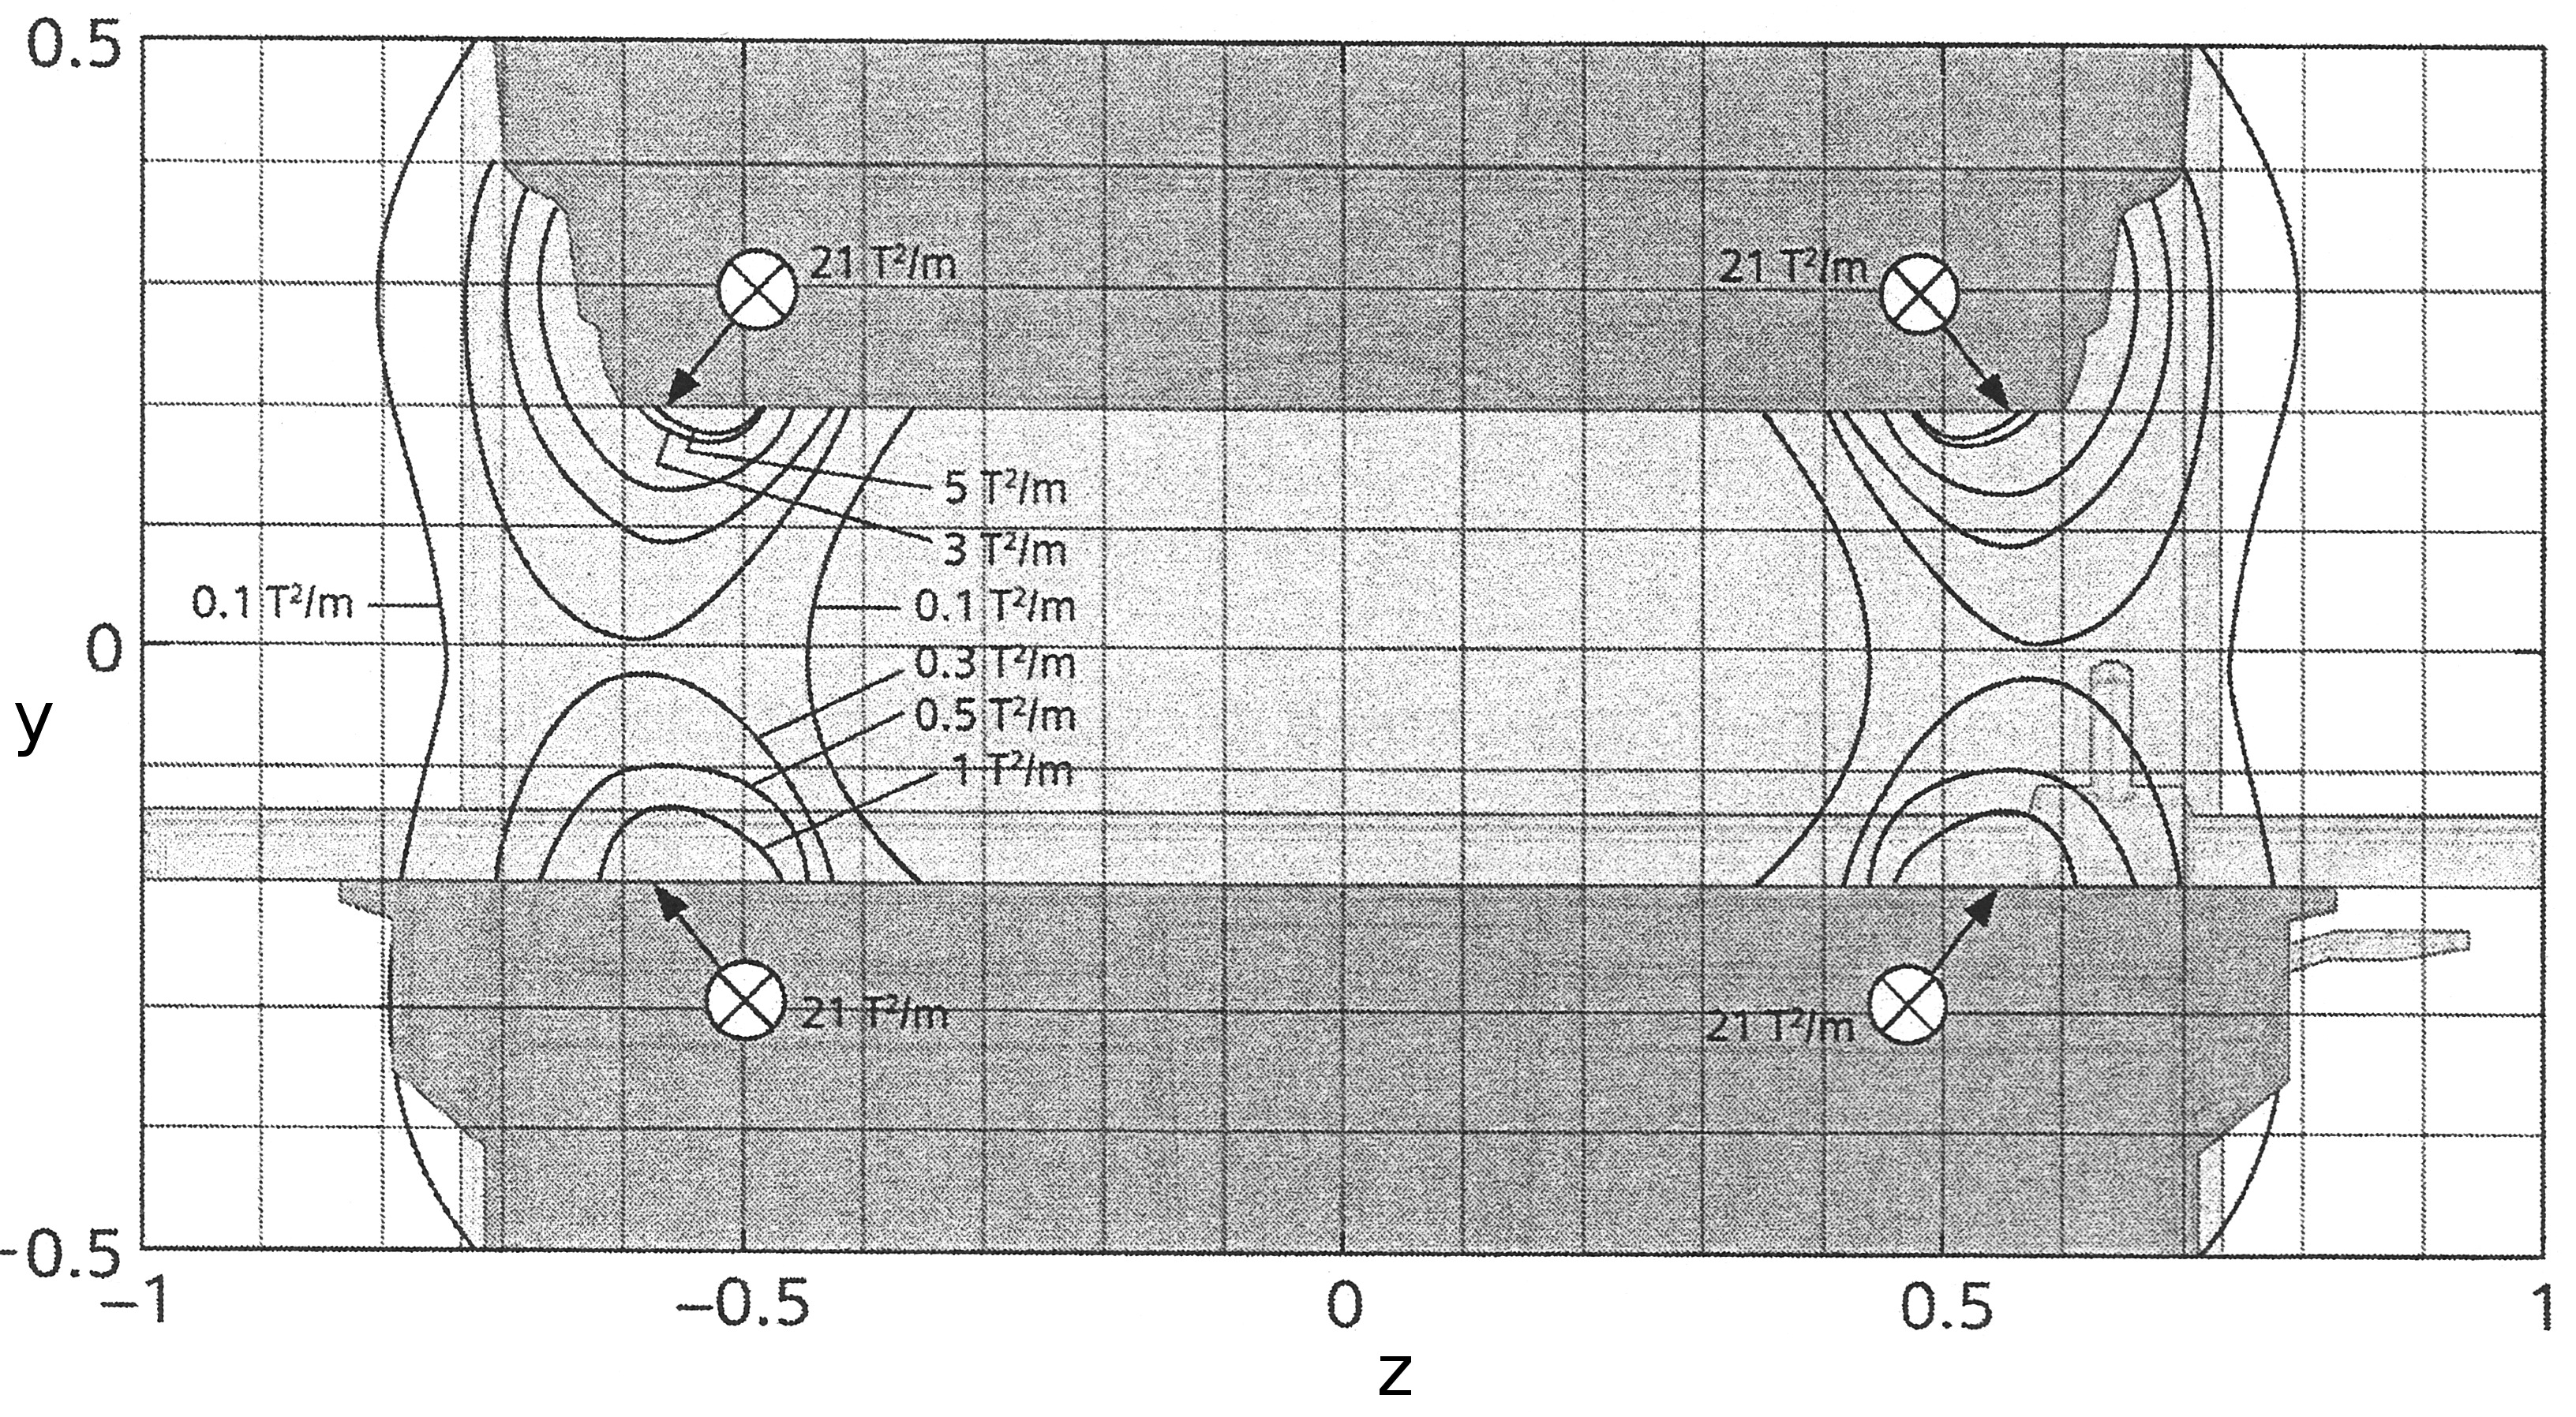
\includegraphics[scale=1.1]{scanner/scanner_gradient-front.jpg}
    \caption[Magnetom C! field gradient\\ front view along x-axis. Image source: \cite{magnetom_handbook}]{Magnetom C! field gradient\\ front view along x-axis (see fig. \ref{fig:scanner_front}). Image source: \cite{magnetom_handbook} (with kind support of Siemens Healthineers)}
    \label{fig:gradient_front}
    \end{figure}

\begin{figure}[!htb]
  	\centering
    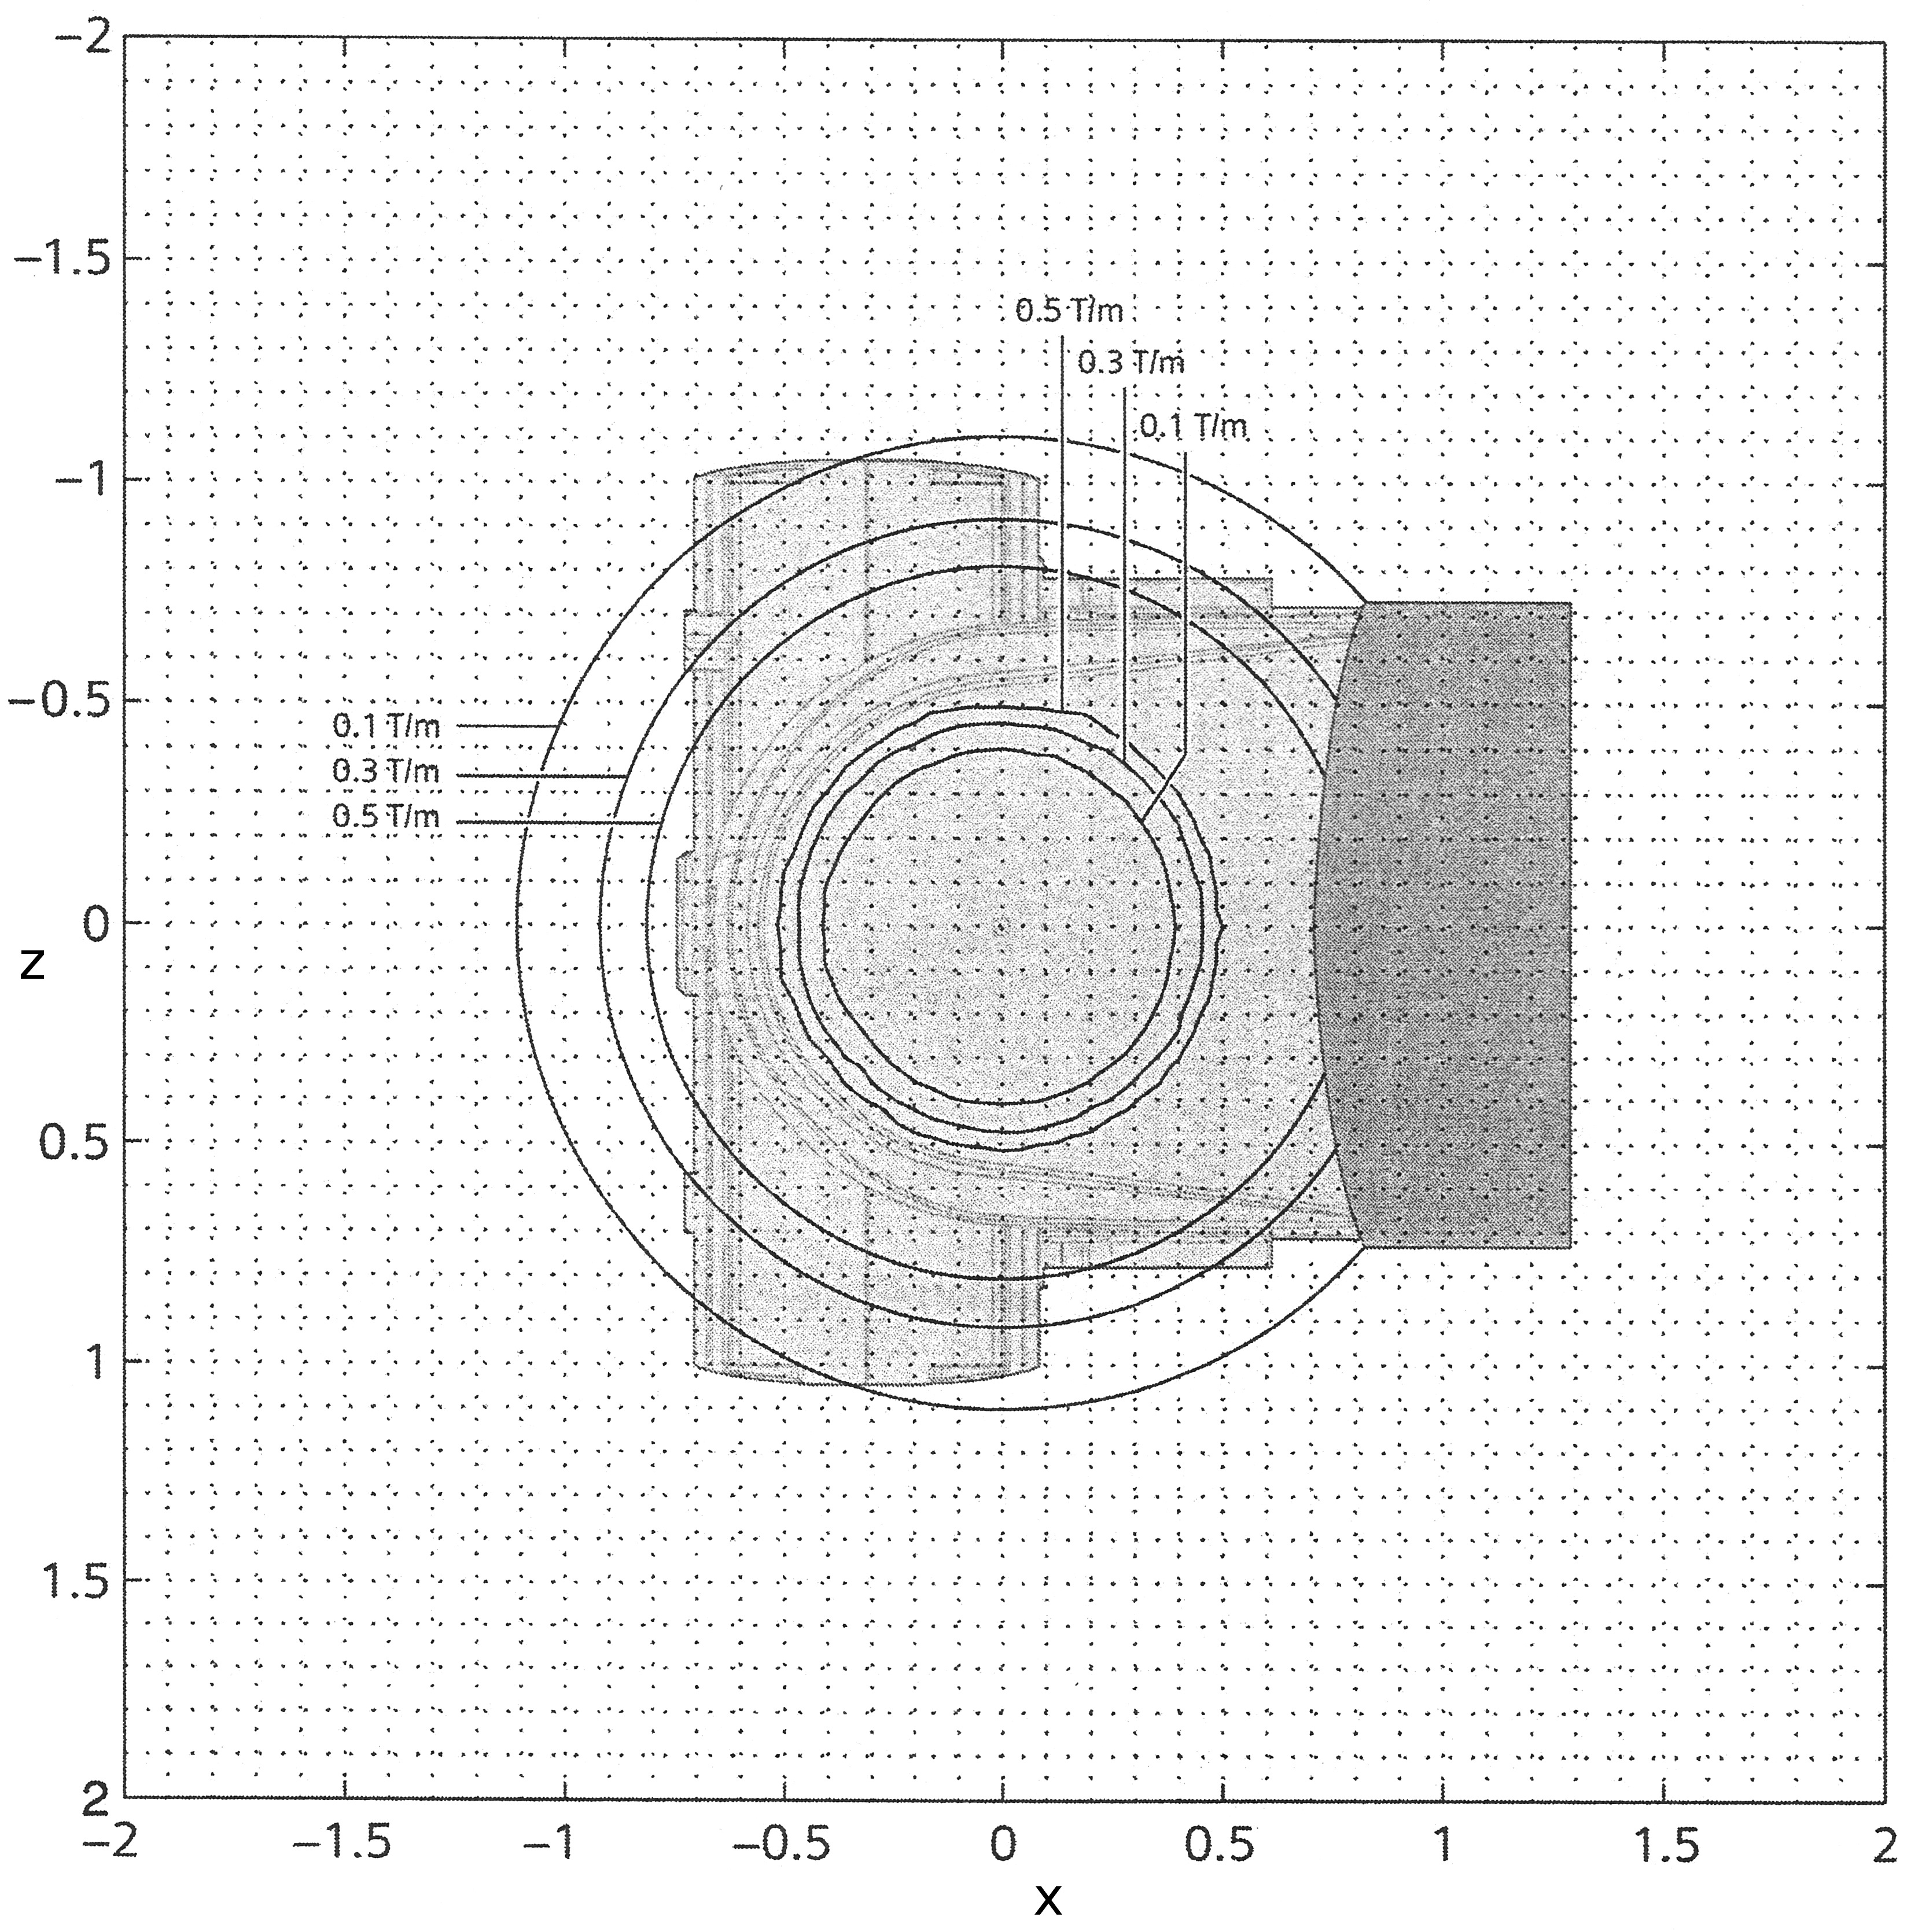
\includegraphics[scale=1.1]{scanner/scanner_gradient-top.jpg}
    \caption[Magnetom C! field gradient\\ top view along y-axis. Image source: \cite{magnetom_handbook}]{Magnetom C! field gradient\\ top view along y-axis (see fig. \ref{fig:scanner_top}). Image source: \cite{magnetom_handbook} (with kind support of Siemens Healthineers)}
    \label{fig:gradient_top}
\end{figure}


\section{Custom build phantom}

To compare images from different scanners and asses occurring distortion, a rigid object with known dimensions is necessary.
Such a 'phantom' is often made from plastics filled with liquids which are easy to handle and typically well seen on MR and CT images.
The AKH's design is made up from an array of replaceable, fillable plastic rods.

\begin{figure}[!htb]
\centering
  \begin{subfigure}[b]{0.1\textwidth}
    
\includegraphics[scale=1]{slicer3D/full_phantom/sagittal_comparison_mr.png}
    \caption{MR}
    \label{fig:sagittal_comparison_mr}
  \end{subfigure}
  \begin{subfigure}[b]{0.1\textwidth}
    
\includegraphics[scale=1]{slicer3D/full_phantom/sagittal_comparison_ct_empty.png}
    \caption{CT}
    \label{fig:sagittal_comparison_ct_empty}
  \end{subfigure}
  \begin{subfigure}[b]{0.1\textwidth}
    
\includegraphics[scale=1]{slicer3D/full_phantom/sagittal_comparison_ct.png}
    \caption{CT}
    \label{fig:sagittal_comparison_ct}
  \end{subfigure}
  \caption[Comparison: MRI only shows filling, CT also the plastic rod and pane]{Comparison (inverted colours): MRI only shows liquid filling, CT also the plastic rod and pane (horizontal black bar crossing middle and right rod);\\ (\textbf{a:}) \textit{MRI} - filled rod, plastic not visible (field of view too small to show entire rod); (\textbf{b:}) \textit{CT} - empty rod, plastic visible; (\textbf{c:}) \textit{CT} - filled rod, plastic and filling visible.}
  \label{fig:sagittal_comparison}
\end{figure}

\subsection{Frame and rods}

The phantom was build to fit the largest available rigid coil for the MR scanner.
Three parallel acrylic glass panes in the shape of the coil serve as a frame for the plastic rods.
In the middle an empty area was reserved for an optional additional smaller phantom (not used for this work).
Figure \ref{fig:rendered_CT} shows a rendered CT picture of the phantom. See also figure \ref{fig:axial_CT_pane} showing a CT image of one pane (with no rods inserted). \\
More than 300 plastic rods (length: $50\,cm$, outer diameter: $8\,mm$, inner diameter: $4\,mm$, volume: approx. $6\,ml$) could be placed in the phantom.
See figure \ref{fig:rod_schematic} for a schematic sketch of one rod.
The bottom part of each rod was sealed with a glued plastic plug, the top could be closed with a plastic screw.
Frame and rods were already build and assembled before the author started working on this project.

Additionally, to the rods which would be used to assess the distortion, a number of vitamin pills\footnote{soft gel capsules containing vitamin E and A \cite{pillshere}} were attached to the frame as reference markers (see figure \ref{fig:pills}).
These pills are visible in both CT and MR images and were used to align them (see section \ref{sec:prep}).
This way there is another way of checking the alignment during the prototyping process in addition to the rods.


\begin{figure}[!bp]
\centering
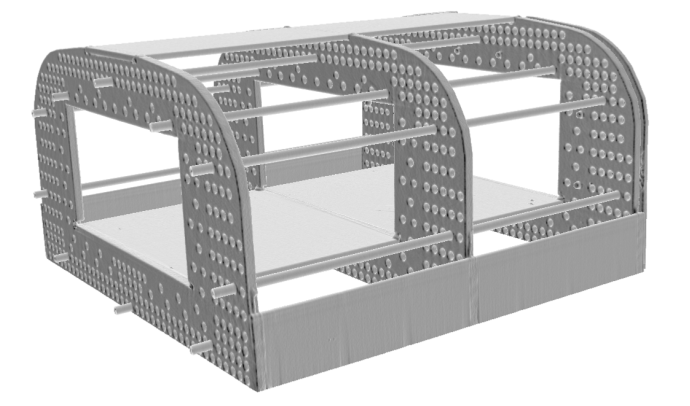
\includegraphics[width=\textwidth]{rendered/rendered_CT.png}
\caption{Rendered CT image of phantom. Image source: Courtesy Piotr Andrzejewski (unpublished data)}
\label{fig:rendered_CT}
\end{figure}

%\begin{figure}[!bp]
%\centering
%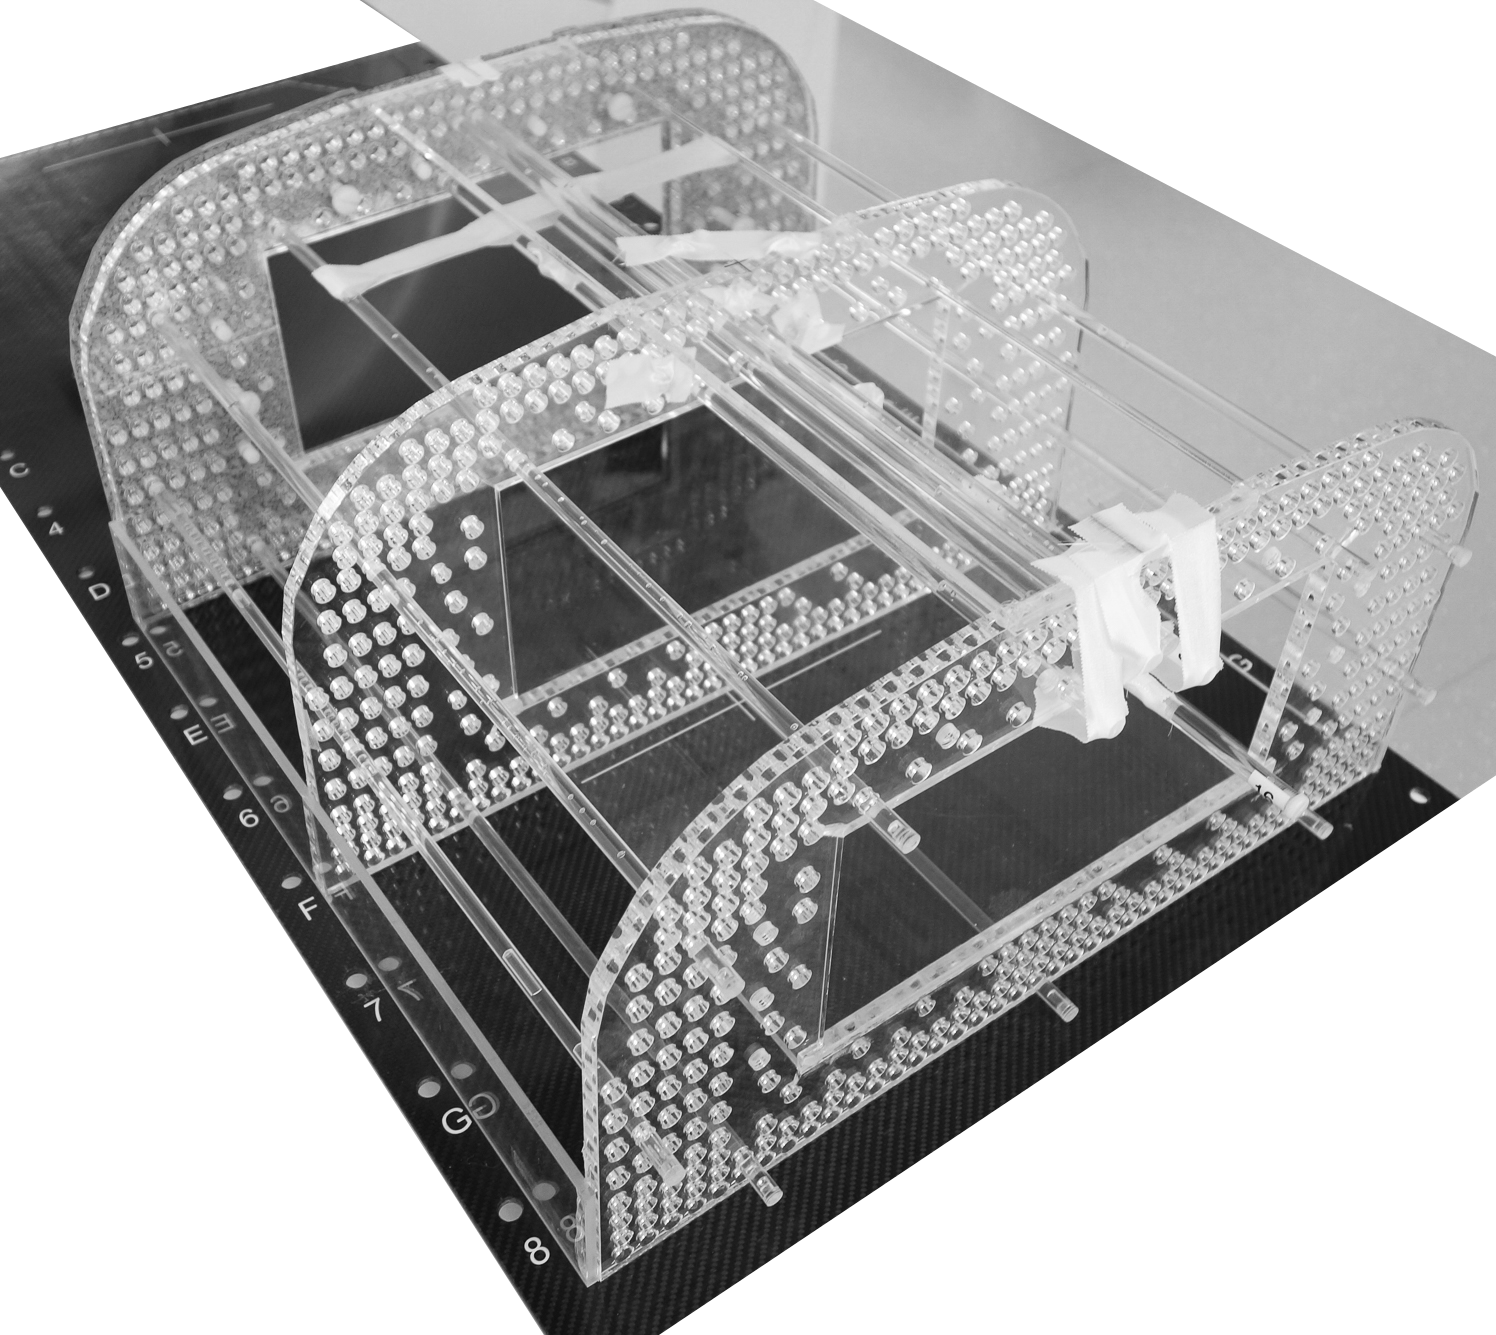
\includegraphics[width=\textwidth]{photo/ph3_CT-scanner.png}
%\caption{Picture of phantom on CT table}
%\label{fig:photo_ph3}
%\end{figure}

\begin{figure}[!tbp]
\centering
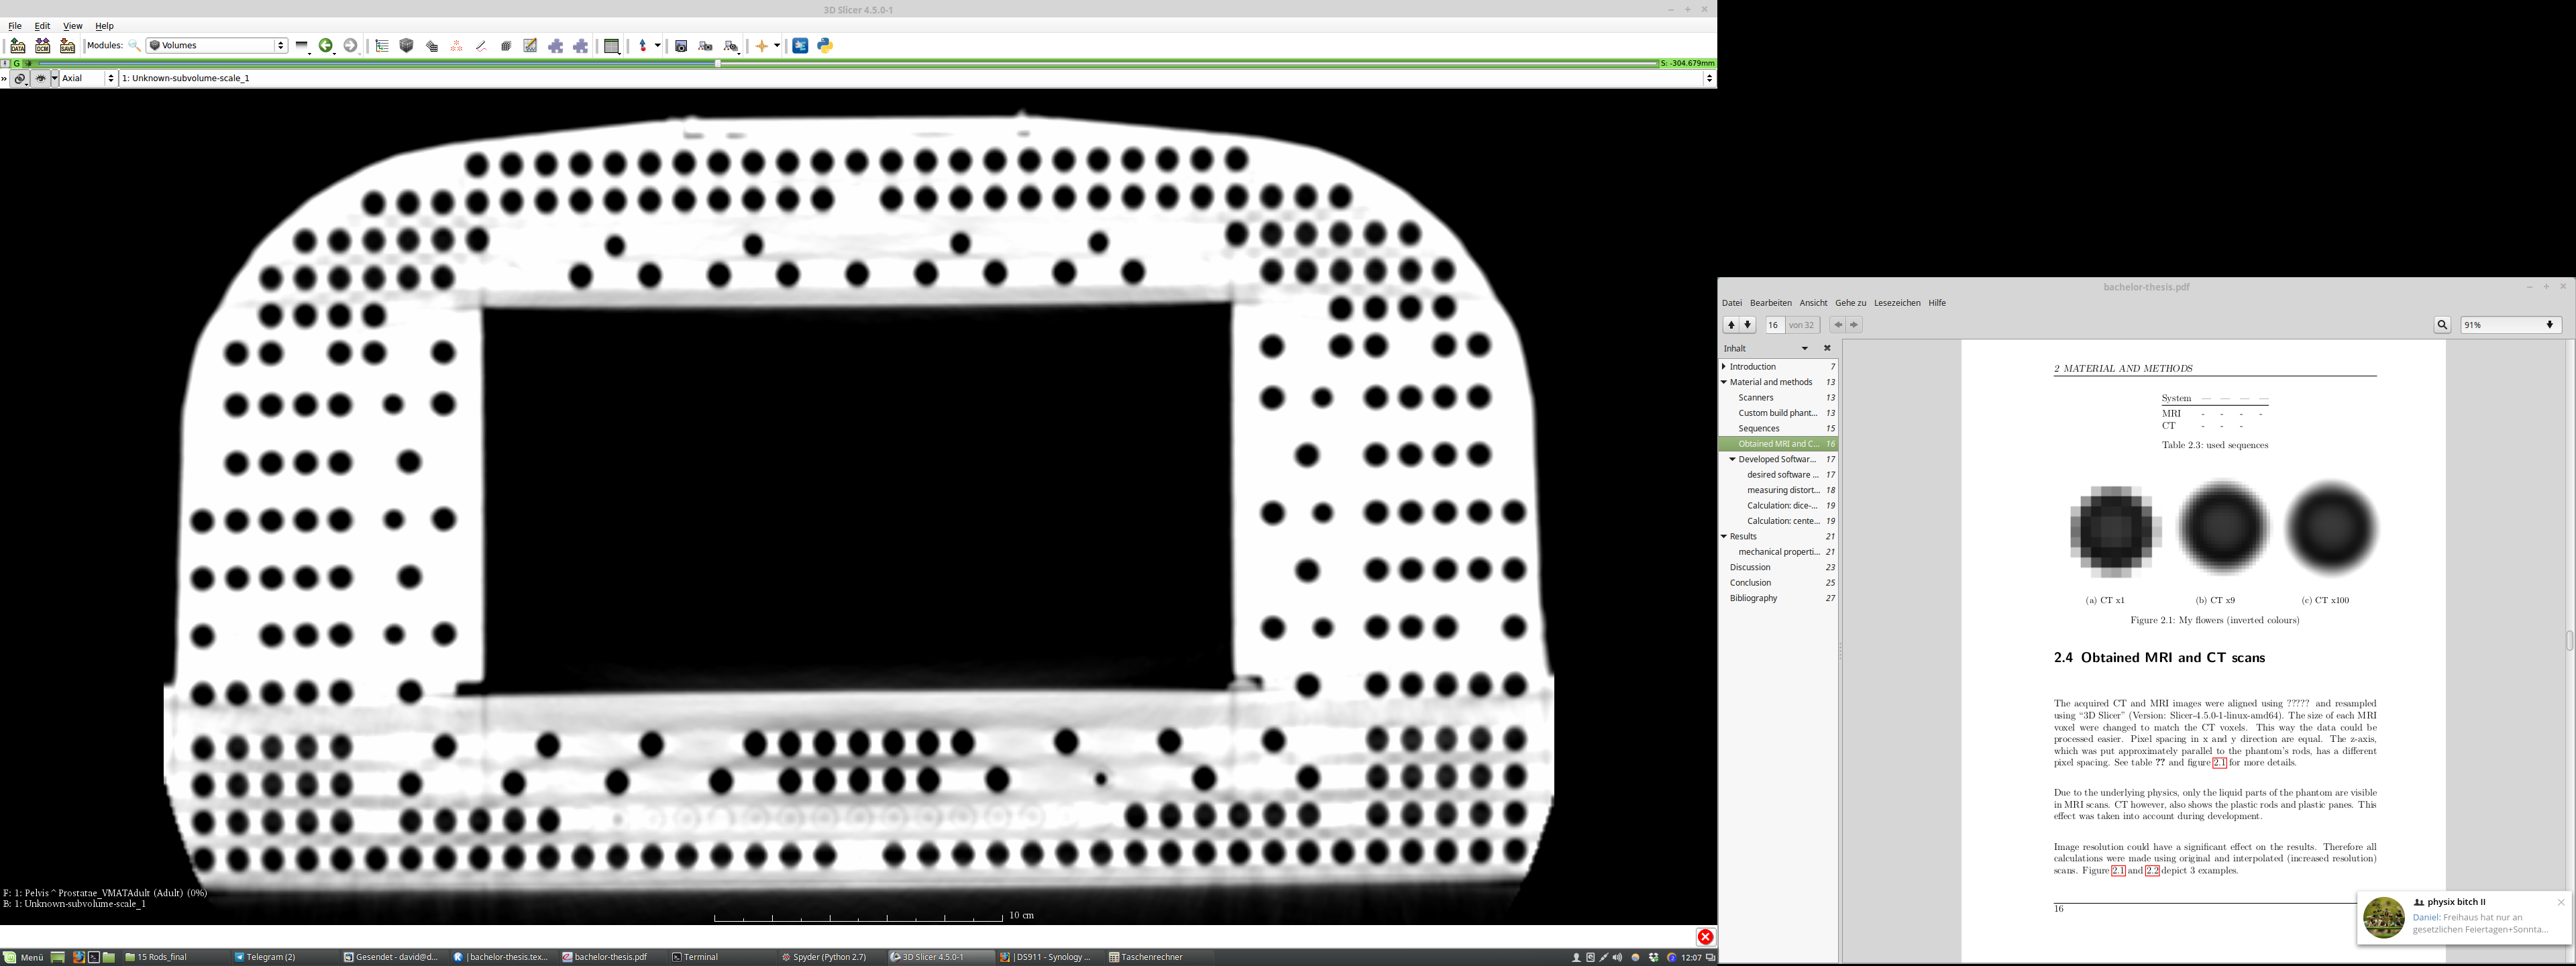
\includegraphics[width=\textwidth]{slicer3D/full_phantom/axial_CT_pane.png}
\caption[Axial view of one of the plastic panes making up the frame of the phantom.]{An axial view of one of three plastic panes that make up the frame of the phantom. This scan shows how the pane looks like with no rods inserted. A little 'x' in one of the holes slightly to the right of the lower part of the pane marks where rod \#5 was inserted later for imaging (see section \ref{sec:rod5}); a little 'z' in the centre of the upper area indicates where rod \#16 was inserted for another imaging sequence (see section \ref{sec:rod16}).}
\label{fig:axial_CT_pane}
\end{figure}

\begin{figure}[!tbp]
\centering
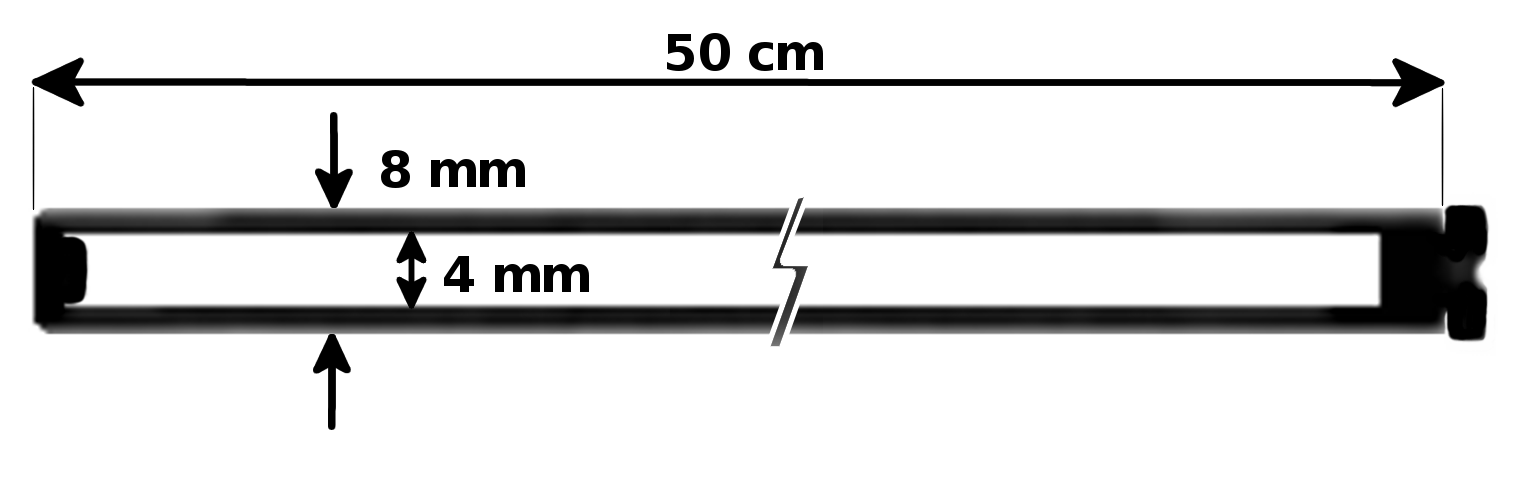
\includegraphics[width=0.8\textwidth]{slicer3D/full_phantom/rod_schematic.png}
\caption[Schematic of an empty plastic rod.]{A schematic of an empty plastic rod as they are used for the phantom (inverted colours). On the left the rod ends with a glued plastic stopper, on the right hand side a plastic screw seals it. The figure does not show true proportions.}
\label{fig:rod_schematic}
\end{figure}


\begin{figure}[!thb]
\centering
  \begin{subfigure}[b]{0.45\textwidth}
  \centering
    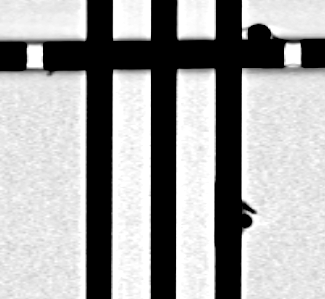
\includegraphics[scale=0.6]{slicer3D/pills_here/pills_CT.png}
    \caption{CT scan}
    \label{fig:pills_CT}
  \end{subfigure}
  \begin{subfigure}[b]{0.45\textwidth}
  \centering
      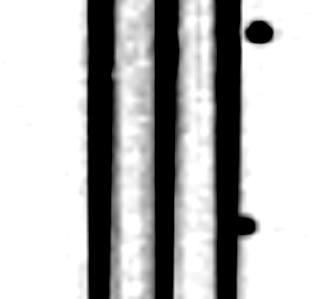
\includegraphics[scale=0.6]{slicer3D/pills_here/pills_MRI.png}
    \caption{MR scan}
    \label{fig:pills_MR}
  \end{subfigure}
  \caption[Coronal CT and MR images showing rods and 2 attached vitamin-e pills]{CT (a) MR (b) coronal images (inverted colours) showing rods and 2 attached vitamin-e pills visible on the right hand side of the rods. In the CT scan the plastic pane and adhesive tape used to hold the pills in place are also visible.}
  \label{fig:pills}
\end{figure}

\clearpage

\subsection{Rod fillings}

For this study 17 different liquids were produced to be tested as possible fillings.
They are listed in Table \ref{tab:solutions}.


\begin{table}[!hbt]
\centering
\caption[The composition of all tested solutions.]{The composition of all tested solutions.\\(components in $g/L$; exception: Primovist in volume-\%)}
\begin{tabular}{@{}l|rrrrrr@{}}
No.   & $NaCl$   & $CuSO_4\cdot5H_2O$          & Soap & Ascorbic Acid & Agar & Primovist [volume-\%]\\
\toprule
\multicolumn{3}{l}{water based:} \\
\#1  &             &                   &      &               &           &		\\
\#2  & 3.6         & 1.96              &      &               &           &		\\
\#3  & 3.6         & 3.92              &      &               &           &		\\
\#4  & 3.6         & 19.6              &      &               &           &		\\
\#5  & 3.6         & 1.96              & 1    &               &           &		\\
\#6  & 3.6         & 1.96              & 5    &               &           &		\\
\#7  & 3.6         & 1.96              & 20   &               &           &		\\
\#8  & 3.6         & 1.96              &      & 0.36          &           &		\\
\#9  & 3.6         & 1.96              &      & 3.6           &           &		\\
\#10 & 3.6         & 1.96              &      & 36            &           &		\\
\#11 & 3.6         &                   &      &               &           & 0.1\%	\\
\#12 & 3.6         &                   &      &               &           & 1\%		\\
\#13 & 3.6         &                   &      &               &           & 10\%	\\
\#14 & 3.6         & 1.96              &      &               &  0.5      &		\\
\#15 & 3.6         & 1.96              &      &               &   20      &		\\
\midrule
\multicolumn{3}{l}{non water based:} \\
\#16 & \multicolumn{2}{r}{Motor Oil:}   & \multicolumn{4}{l}{\textit{Castrol Power1}}      \\
\#17 & \multicolumn{2}{r}{Silicon Oil:} & \multicolumn{4}{l}{\textit{Charge: 15HLVY023}}
\end{tabular}
\label{tab:solutions}
\end{table}


Being closed at one end and having a capillary shape (small diameter) makes it impossible to fill the rods by simply pouring the liquid through the opening.
Instead of adding the fluid at the top, it has to be injected starting at the bottom.
This way the contained air is pushed out by the injected liquid through the opening at the top.
A long, thin plastic tube was inserted and used for injection, leaving enough room for the gas to escape.
Between injections of different liquids, the tube was flushed with \textbf{\#1} (distilled water) or \textbf{\#2} (main component of most solutions).

In order to minimise the amount of gas dissolved, the liquids were brought to boil shortly before injecting. Gas solubility generally decreases with rising temperature \cite{Henry1803, Sander2015}.
After injecting the solution in the rods, they were left to cool down.
Before closing, the rods were topped up completely (no trapped air bubbles).
The oil based liquids, \textbf{\#16} and \textbf{\#17}, were not brought to boil.

\subsection{Handling of bubbles}

On the second day of working with the filled rods the one containing liquid \textbf{\#6} broke (leakage).
It happened when delicately knocking it against on the table while standing upright.
This was intended to mobilise bubbles that sticked to the wall and make them travel vertically to on end of the rod. (see table \ref{tab:bubbles1})
The plastic stopper on the lower end came loose.
The rod containing filling \textbf{\#6} was not replaced.
Consequently, all CT/MR images used to asses signal intensities of the tested solutions show only 16 rods.


\section{Used software applications}

Prior to analysing the data, the scans had to be prepared.
For this task, two applications were used:
\begin{itemize}
\item \textit{MIRADA RTx}: a commercial software solution for both diagnostic imaging and radiation oncology \cite{mirada} was used to align CT and MR images.
\item \textit{3D Slicer}: (Versions: Slicer-4.5.0-1-linux-amd64, Slicer-4.6.2-win-amd64) a "free and open source software package for visualisation and medical image computing". \cite{3DSlicer, Kikinis2012} was used to crop and resample images, quickly read values and visualise the results.
\end{itemize}


\section{Pre-processing MRI and CT scans}
\label{sec:prep}

Figures \ref{fig:rendering1-3}, \ref{fig:rendering4-5} and \ref{fig:resample} show the most important stages in the image processing work flow performed to prepare the data for the developed script.

\begin{enumerate}[label=\textbf{Step \arabic*}]
\item After loading the CT and MR scan into \textit{MIRADA}, they were aligned using the vitamin-e pills, yielding maximum overlap in the centre of the image.
\item Next, as the MR image had a lower resolution than the CT scan, the MR scan was resampled.
Its voxel size were changed to match the CT voxels and both scans exported.
\item Both layers (MRI and CT) were loaded into \textit{3D Slicer}.
\item Its module 'annotations' was used to set a new region of interest (ROI) to include only a single rod.
\item With the module called 'crop volume' (setting: voxel based cropping) the scans were reduced to show only the selected ROI.
\item Using the module 'resample scalar volume' a number of interpolated (setting: 'bspline') higher resolution pairs (CT/MRI) were created.
\item All new pairs and the cropped original CT/MRI pair were exported with 'create a dicom series' and saved in a separate folder each.
\end{enumerate}
\vspace*{0.5cm}

After this procedure a number of pairs based on the original CT and MRI were available, all of which had the same number of slices along the z-axis parallel to the phantom's rods.
They only differ in the number of pixels making up each slice, their resolution varying from the original up to a hundred times finer.
Each pair (CT/MRI) has the same pixel spacing (and resolution) in x and y direction.
See table \ref{tab:spacing} for more details.
Figure \ref{fig:resample} depicts 3 CT/MR scans of a single rod (axial) with different resolutions.
"x1" stands for the original CT scan resolution (MRI resampled to match).
"x4" is a resolution caused by 1 pixel being split in 4 smaller pixels, "x9" in 9, and so on and so forth.
For better visibility, images shown as figures in this work are printed with inverted colours.
Dark pixels have a high density/intensity value, white pixels are equivalent to air (low density/intensity).

\begin{table}[!htb]
\centering
\caption[Pixel Spacing and resample rates.]{Pixel Spacing and resample rates (rounded values) [$mm$].}
\begin{tabular}{l|l|l|l}
resample factor  & z (not affected) &  y (same as x) & x \\
\toprule
x1     & 0.60 & 0.98	& 0.98	\\
x4     & 0.60 & 0.49	& 0.49	\\
x9     & 0.60 & 0.33	& 0.33	\\
x25    & 0.60 & 0.2 	& 0.2	\\
x100   & 0.60 & 0.1 	& 0.1
\end{tabular}
\label{tab:spacing}
\end{table}

\begin{figure}[!thb]

  \begin{subfigure}[b]{0.45\textwidth}
    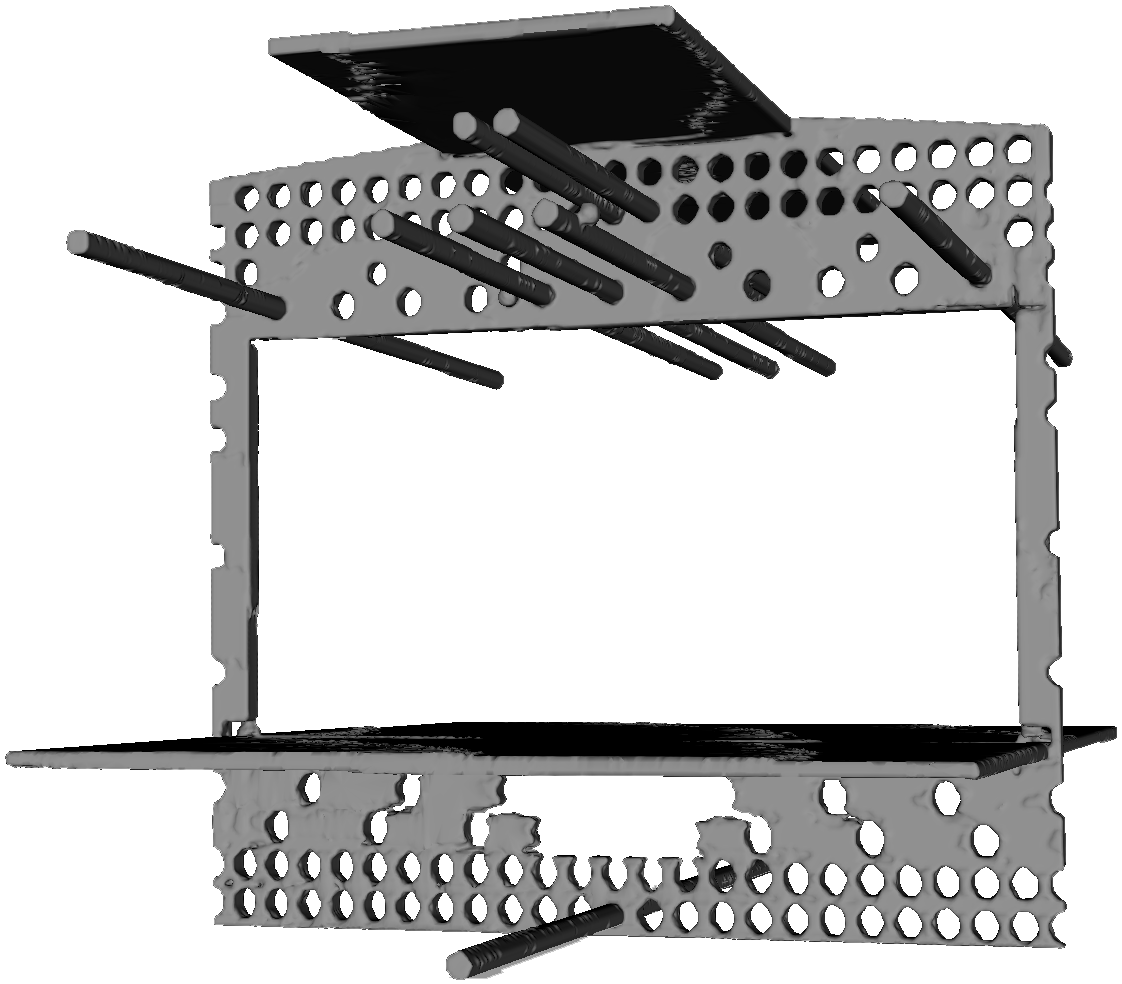
\includegraphics[scale=.2]{rendered/CT-full.png}
    \caption{CT}
    \label{fig:CT_full}
  \end{subfigure}
  \hfill
  \begin{subfigure}[b]{0.45\textwidth}
    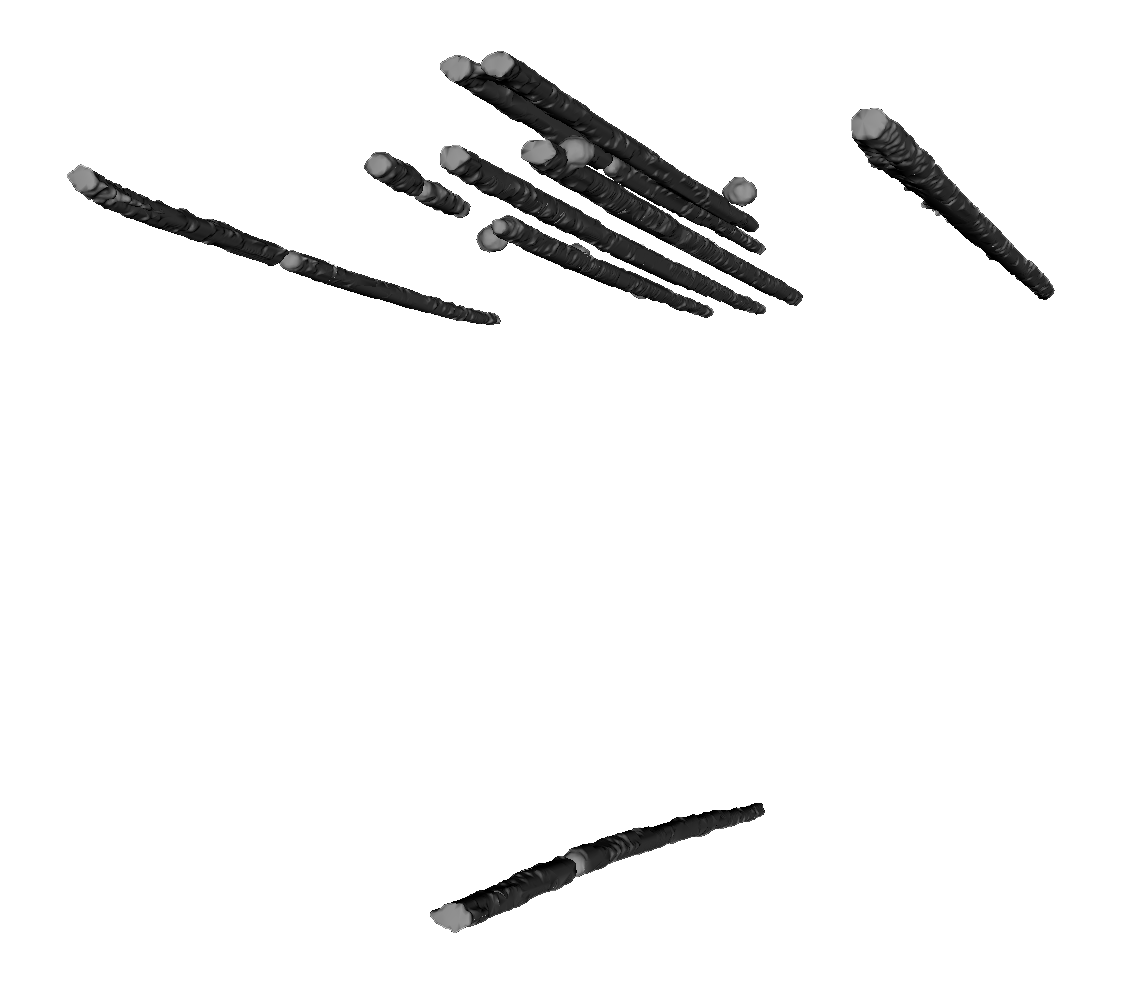
\includegraphics[scale=.2]{rendered/MR-full.png}
    \caption{MR}
    \label{fig:MR_full}
  \end{subfigure}
  \caption{Rendered CT/MR image of phantom after steps 1-3 of pre-processing.}
  \label{fig:rendering1-3}
\end{figure}
  
\begin{figure}[!thb]
  \begin{subfigure}[b]{0.45\textwidth}
    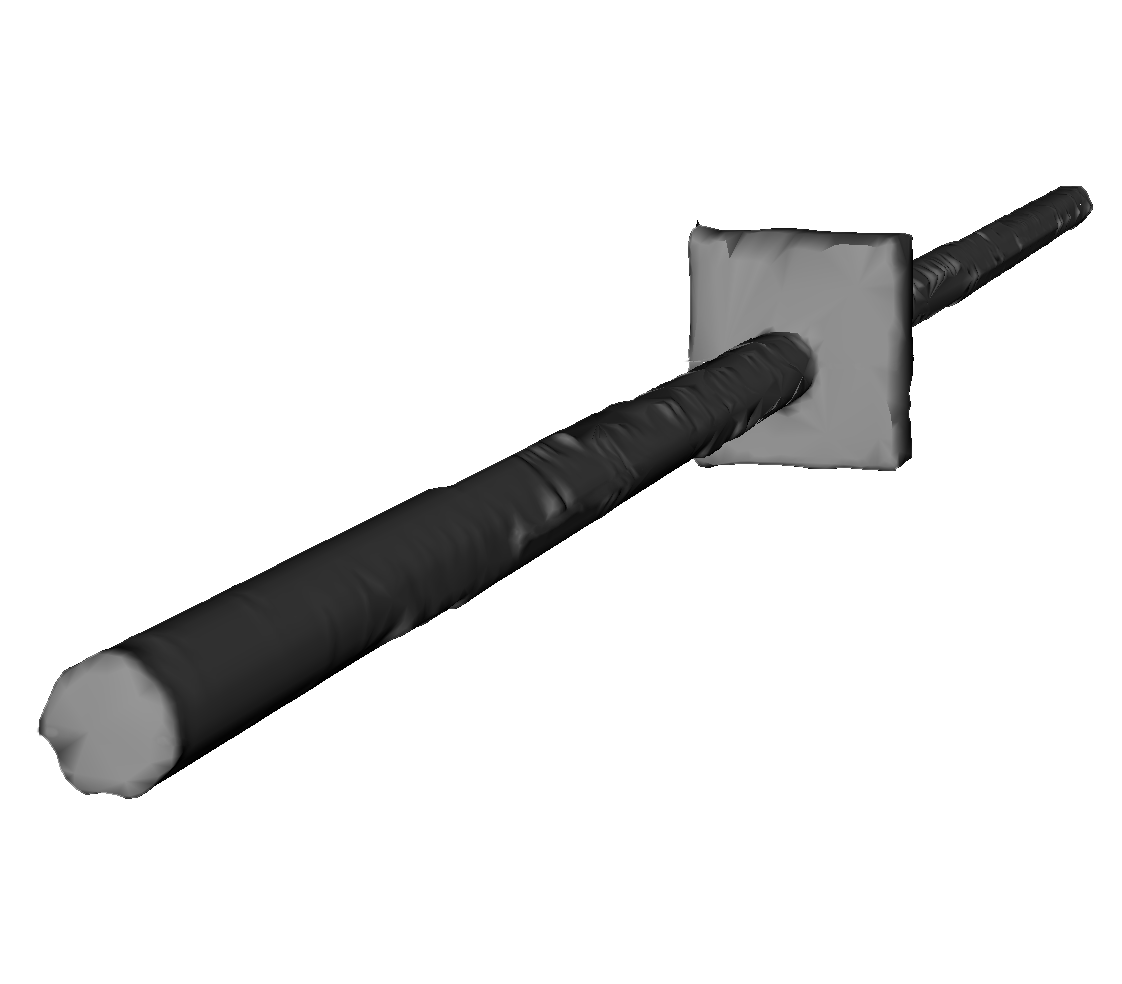
\includegraphics[scale=.2]{rendered/CT-rod.png}
    \caption{CT}
    \label{fig:CT_rod}
  \end{subfigure}
  \hfill
  \begin{subfigure}[b]{0.45\textwidth}
    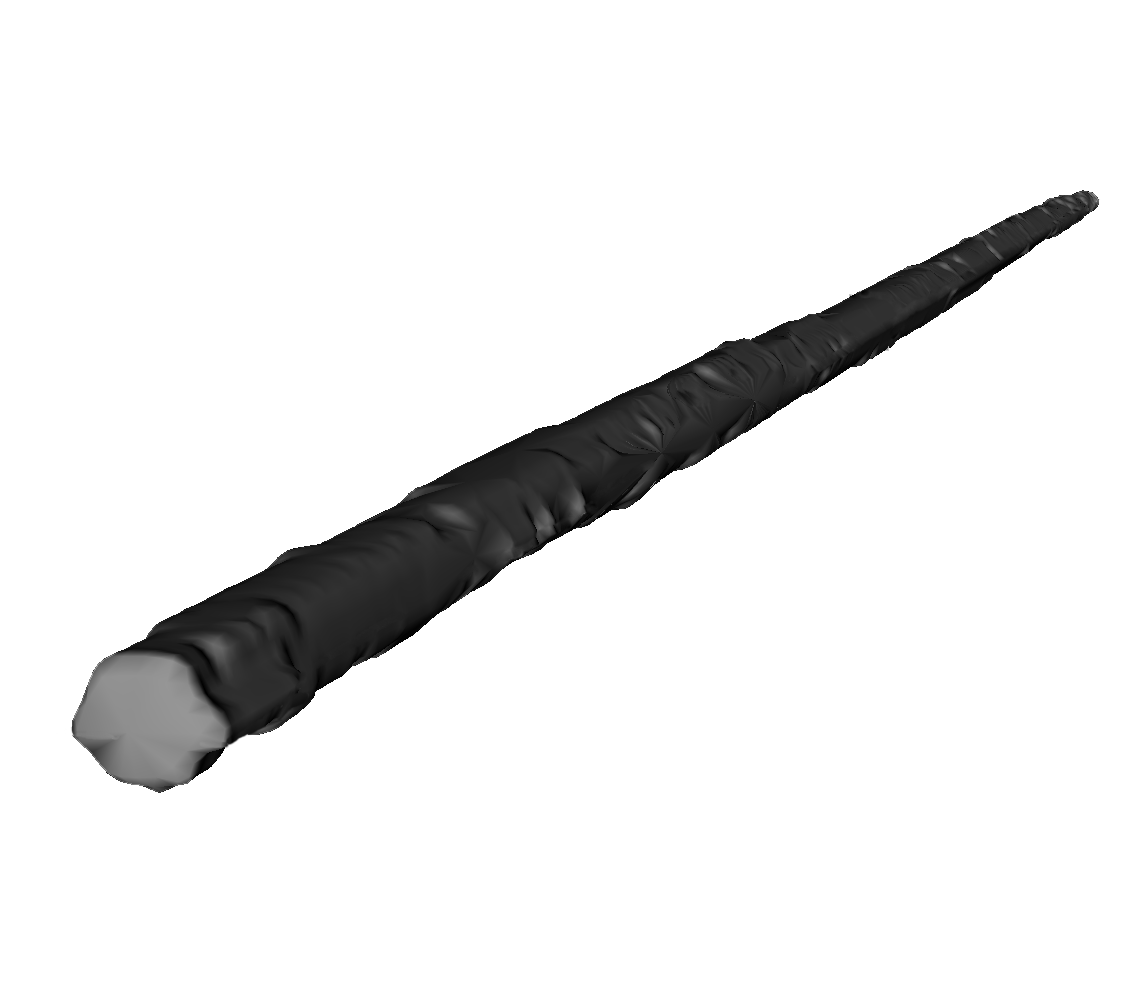
\includegraphics[scale=.2]{rendered/MR-rod.png}
    \caption{MR}
    \label{fig:MR_rod}
  \end{subfigure}
  
  \caption{Rendered CT/MR image of phantom after steps 4 and 5 of pre-processing.}
  \label{fig:rendering4-5}
\end{figure}

\begin{figure}[!thb]
  \begin{subfigure}[b]{0.32\textwidth}
    
\includegraphics[scale=.11]{slicer3D/profiles/CT_x1.png}
    \caption{CT x1}
    \label{fig:CT_x1}
  \end{subfigure}
  \hfill
  \begin{subfigure}[b]{0.32\textwidth}
    
\includegraphics[scale=.11]{slicer3D/profiles/CT_x9.png}
    \caption{CT x9}
    \label{fig:CT_x9}
  \end{subfigure}
    \hfill
  \begin{subfigure}[b]{0.32\textwidth}
    
\includegraphics[scale=.11]{slicer3D/profiles/CT_x100.png}
    \caption{CT x100}
    \label{fig:CT_x100}
  \end{subfigure}
  \begin{subfigure}[b]{0.32\textwidth}
    
\includegraphics[scale=.11]{slicer3D/profiles/MR_x1.png}
    \caption{MRI x1}
    \label{fig:MRI_x1}
  \end{subfigure}
  \hfill
  \begin{subfigure}[b]{0.32\textwidth}
    
\includegraphics[scale=.11]{slicer3D/profiles/MR_x9.png}
    \caption{MRI x9}
    \label{fig:MRI_x9}
  \end{subfigure}
    \hfill
  \begin{subfigure}[b]{0.32\textwidth}
    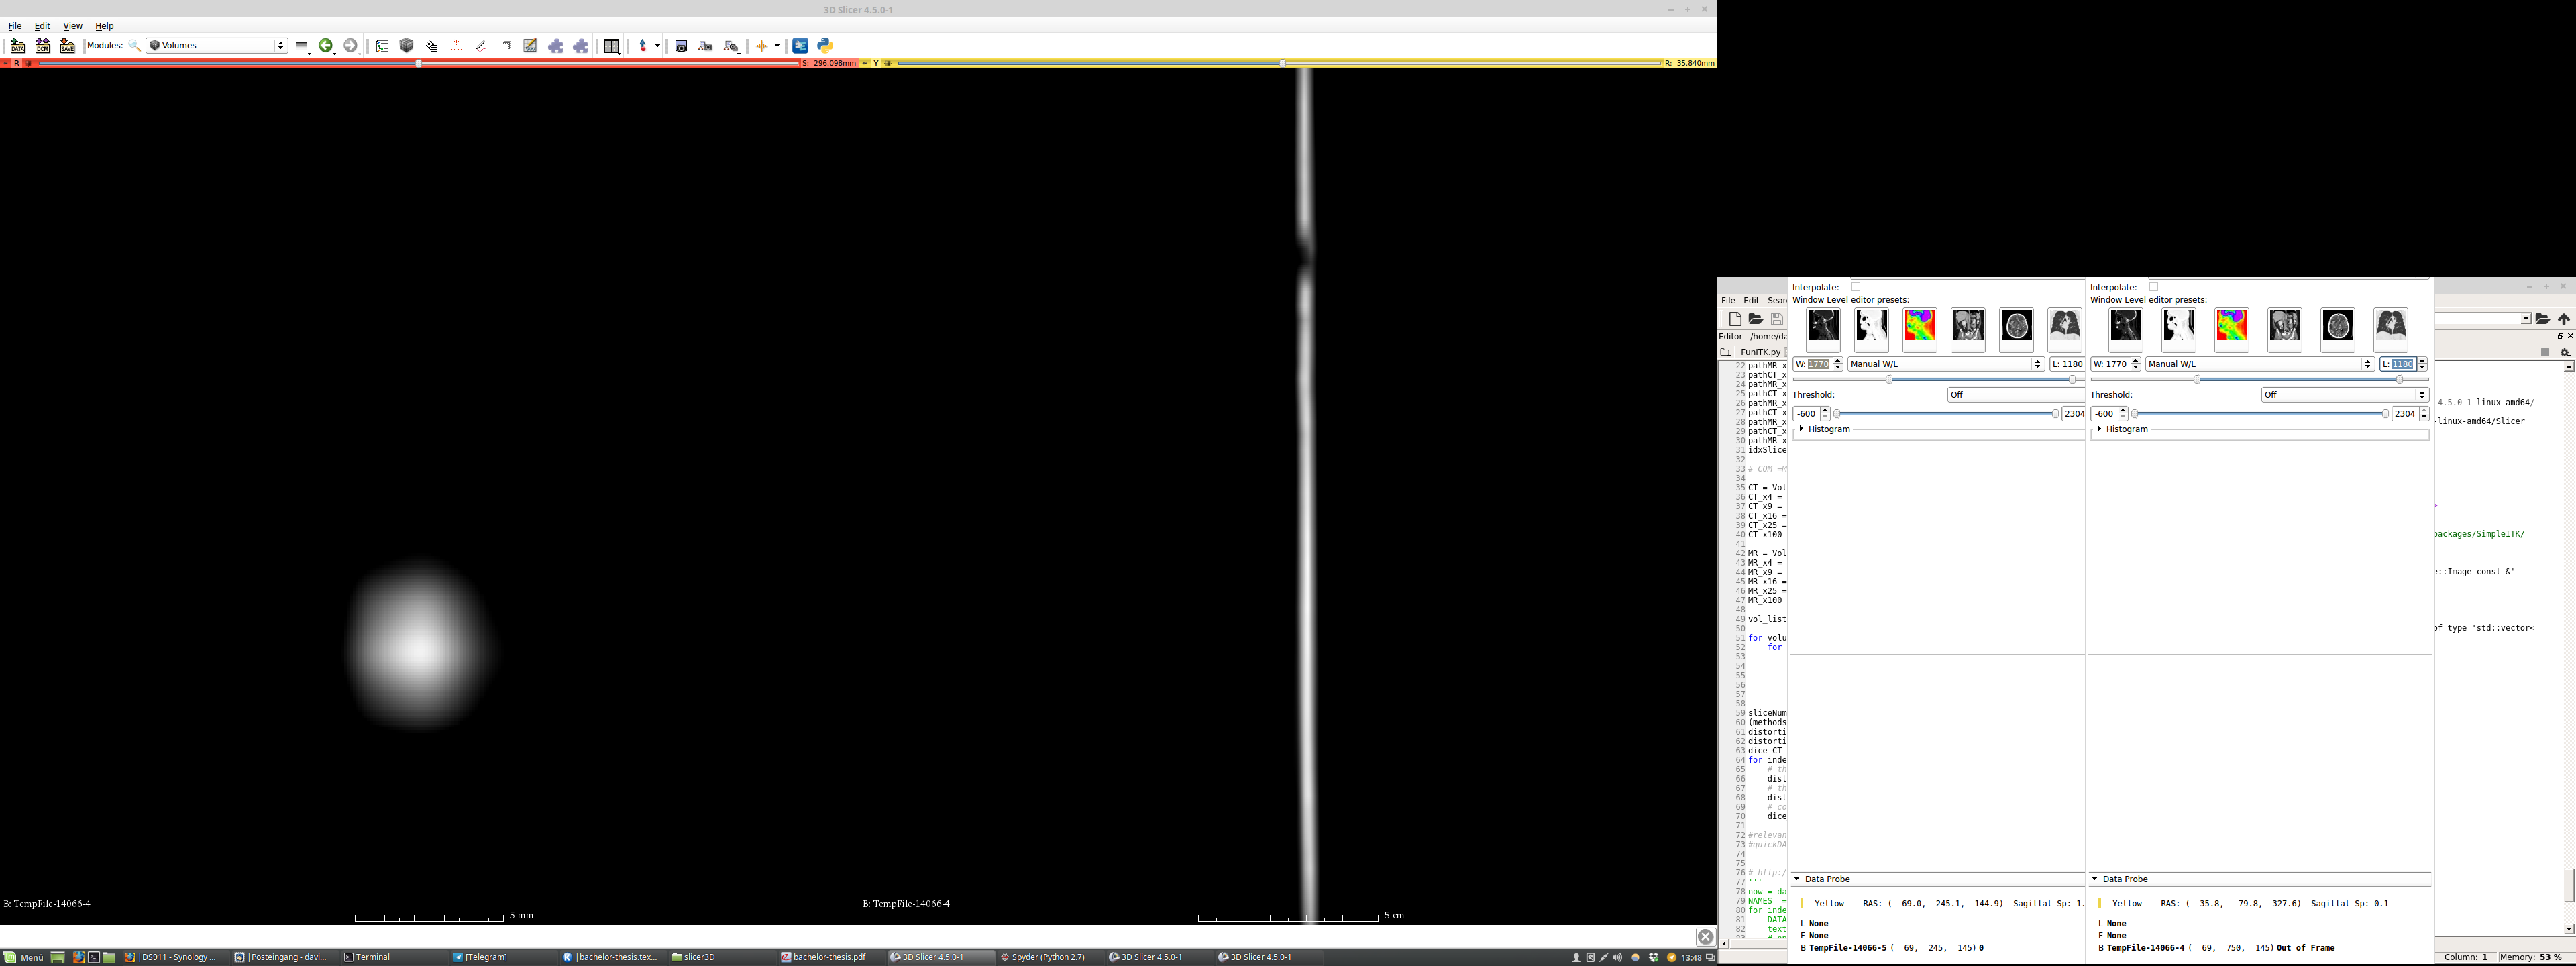
\includegraphics[scale=.11]{slicer3D/profiles/MR_x100.png}
    \caption{MRI x100}
    \label{fig:MRI_x100}
  \end{subfigure}
  \caption[Rendered image of phantom after steps 4 and 5 of pre-processing.]{CT/MRI axial images of the same rod (filling \#5, inverted colours) after steps 6 and 7. The images on the very left show the original (CT) resolution, the resolution of those in the middle and the right were increased by resampling (9 times and 100 times finer);\\ pixel lengths: x1 $\rightarrow 0.98\, mm$, x9 $\rightarrow0.33\, mm$, x100 $\rightarrow0.1\, mm$}
  \label{fig:resample}
\end{figure}
\clearpage

\section{Developed software tool}
% conda create --name snowflakes python=2.7 SimpleITK Spyder
% source activate snowflakes
% spyder

In order to asses the distortion of the MR scanner, a software tool was programmed.
It is written in Python 2.7 and uses the \textit{SimpleITK} package to read and process \textit{DICOM} ("\textit{Digital Imaging and Communications in Medicine}") files. \cite{Python, DICOM}
\textit{SimpleITK} is a object-oriented "C\texttt{++} library with wrappers for Python, Java, CSharp, R, Tcl and Ruby". \cite{SimpleITK, SimpleITK_started} Its versatility is one of the reasons why this approach was favoured.
It is a simplified layer built on top of the National Library of Medicine Insight Segmentation and Registration Toolkit (ITK). SimpleITK is also used by Applications like \textit{3D Slicer}.
Documentation and code examples of SimpleITK can be found at \cite{InsightSoftwareConsortium, Kyriakou-SimpleITK}
An alternative way to handle DICOM data in Python would be Pydicom. \cite{Pydicom, Kyriakou-Pydicom-VTK} 

This is an extensive list of python packages used to process data after using 3D Slicer:
\begin{itemize}
 \item SimpleITK
 \item numpy
 \item scipy
 \item matplotlib.pyplot \cite{Hunter2007}
 \item skimage.draw
 \item datetime
 \item os
\end{itemize}


\subsubsection{Capabilities - Overview}

The developed software tool is not able to automatically detect individual rods in a CT or MR scan depicting the whole phantom.
Instead the acquired 3D images have to be cropped so they include only a single rod (see section \ref{sec:prep}).

The python script can be used to:
\begin{itemize}
% \item de-noise the image data
 \item separate bright areas which are not connected ('masking' might be used as future method to automatically detect individual rods)
 \item find and mark slices which show irregularities
 \item calculate the centroid coordinates along the rod
 \item measure the local distortion described by the
  \subitem location shift (refered to as "warp")
  \subitem dice coefficient (the "DC" refers to an object's roundness)
 \item visualise individual rod slices
 \item plot the average/peak brightness, warp, or \texttt{DC} along the rod
 \item write warp and \texttt{DC}  for each slice in a combined ".txt" file
 \item export a rod shaped scan where the pixel values reflect the distortion occurring in each slice instead of their brightness as a ".mha" file (useful for visualisation, see figure \ref{fig:colour-map}).
\end{itemize}


\subsubsection{Measuring distortion}

Since the rods have a cylindrical shape, distortion can only be assessed in radial direction.
The z-axis is parallel to the rods, x and y are radial.
Ideally, each slice (z = const.) should depict the bright circular profile of the liquid (and of the plastic rod in CT) surrounded by black pixels (air).
\\
Two phenomena were chosen to reflect the amount of distortion occurring in each slice of the MR scans.
The distance which the rod appears to be shifted in the MRI slice compared to the CT slice is referred to as "warp".
The rod's deformation (deviation from circular profile) is described using the dice-coefficient "\textit{DC}" (also known as Sorensen-Index).


\subsection{Calculation: dice coefficient (DC)}
\label{sec:DC}

The \texttt{DC} was chosen as indicator for the deviation from a circular profile.
The implementation as python function is based on the open source python package "Medpy". \cite{MedPy} A part of its module called "metric" was adapted. \cite{MedPy_dc-code}\\


The calculation of the \texttt{DC} is performed for each slice individually.
Additionally, to asses the overall distortion occurring along the rod, the average of all those values is also saved.
As this aspect of distortion does not need a reference scan, the \texttt{DC} is measured for CT and MR images separately.
The dice coefficient or Sorensen index \cite{MedPy_dc-doc} is defined as:
\begin{align}
\label{eq:DC}
DC = \frac{2 |A \, \cap \, B|}{|A| + |B|}
\end{align}

Figure \ref{flo:DC} describes the process of calculating the DC.
It compares a binary image (input A) to a circle (reference B).
In a binary image there are only 2 possible pixel values: "0" and "1".
However, in a CT image, values most often lie in a range between -1024 and 1000 or higher.
In order to reduce the original image to a binary image A, the script needs to split the pixels in 2 groups.
A copy of the original picture is created where all pixels with a value above a certain  \texttt{threshold} are set to the value of "1".
These are regarded as part of the rod.
Those which are darker are set to "0".
(See section \ref{sec:COM} for details on how the \texttt{threshold} is calculated).
Ideally, this procedure separates the surrounding dark area from the bright rod by using a suitable \texttt{threshold}.
This way the new binary image A still shows were the rod is, but it lost all information on the actual brightness.

Reference B is a circle with its midpoint typically placed at the centre of mass (COM) of the rod.
The \texttt{COM} is usually calculated using those pixels which exceed the \texttt{threshold}, but weighted with their actual brightness (not using the binary image)

This way the script is supposed to place the reference circle B in the centre of the input image A.
The position of the circle's centre and its radius highly influence the outcome.
If the COM coordinates used to position the reference circle B lie outside of the image (e.g. '-1,-1'), the DC is set to '-1', indicating that no meaningful result could be obtained.

The \texttt{DC} ranges from 0 to 1.
A value of 1 indicates a perfect circular shape.
A low \texttt{DC}, on the other hand, means the shape differs greatly from a circle and could be caused by many things such as:
little overlap (e.g. a ring or crescent shape); a very dark image hindering delineation of the rod from background; a small circle with a radius close to a only a few pixels.

The obvious choice for the radius of the reference circle B is to use the size of the physical rod/liquid as it is should be visible on the scan.
For CT images this would be $4\,mm$ (outer diameter of the plastic rod), for MR images it would be $2\,mm$ (inner diameter of the plasic rod, equivalent to the diameter of enclosed liquid).
The script calculates the \texttt{DC} using various radii close to those values and returns the result yielding in the highest average \texttt{DC} for the whole rod.

\subsubsection{Using the CT COM}
Alternatively, the DC fo the MR scan can be calculated with the reference circle B placed in the COM of the corresponding CT image.
This value could be regarded as a combined distortion guide number as it is influenced by the COM shift and the deformation simultaneously.
One should bear in mind, though, that the meaning of it is neither equivalent to a real \texttt{DC} nor to the warp and should be interpreted with caution.\\

If the CT COM is far from the MR image, A and B have little overlap resulting in a small \texttt{DC}.
As the implemented \texttt{DC} calculation tries a variety of radii, the circle B could, theoretically, always be chosen big enough to have some overlap with the binary image A.
However, as B grows, A will stay the same.
Therefore, only a fraction of B will contribute to the overlap and the rest will counter-act the benefits (see equation \ref{eq:DC}).
Consequently, the DC would become so small that the script will choose a smaller radius for B.


% Define block styles
\tikzstyle{blockb} = [rectangle, draw, fill=blue!15, text width=18em, text centered, minimum height=4em]
\tikzstyle{cloud} = [draw, ellipse,fill=red!20, text width=12em, text centered, minimum height=5em]
\tikzstyle{block} = [rectangle, draw, fill=green!10, text width=14em, text centered, rounded corners, minimum height=4em]
\tikzstyle{puffs} = [cloud, cloud puffs=13.5, minimum width=4cm, minimum height=1.5cm, align=center, fill=green!10]
\tikzstyle{blocky} = [rectangle, draw, fill=yellow!10, text width=14em, text centered, minimum height=4em]
\tikzstyle{decisionr} = [diamond, draw, aspect=3, fill=red!20, text width=18em, text badly centered, node distance=2.5cm, inner sep=0pt]
\tikzstyle{decisiong} = [diamond, draw, aspect=2, fill=green!10, text width=4.5em, text badly centered, node distance=2.5cm, inner sep=0pt]
\tikzstyle{decisiony} = [diamond, draw, aspect=3, fill=yellow!10, text width=10em, text badly centered, node distance=2.5cm, inner sep=0pt]
\tikzstyle{line} = [draw, very thick, color=black!80, -latex']
%\tikzstyle{cloud} = [draw, ellipse,fill=red!20, text width=14em, node distance=2.5cm, minimum height=2em]


\begin{figure}[!htb]
    \centering
	\begin{tikzpicture}[node distance = 4cm, auto]
    % Place nodes
    \node[] (img) {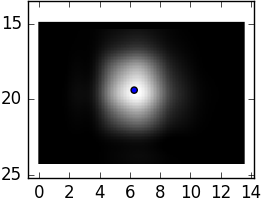
\includegraphics[scale=0.8]{python/ph2/dice_flow/ph2_MR_x100_img@200.png}};
    \node [blockb, below of=img, yshift=0.5cm, text width=10em] (img_t) {\texttt{original image}};
    \node [blockb, below of=img_t, yshift=1cm, xshift=-4cm, text width=16em] (binary_t) {\texttt{binary input image A}:\\pixels where original image is darker than \texttt{threhold} are set to \texttt{0}\\ the others are set to \texttt{1}};
    \node [blockb, below of=img_t, yshift=1cm, xshift=4cm, text width=16em] (circle_t) {\texttt{reference circle B}:\\with centre at \texttt{COM} of \texttt{original image}};
    \node[below of=binary_t] (binary) {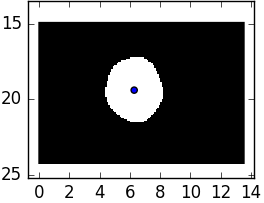
\includegraphics[scale=0.8]{python/ph2/dice_flow/ph2_MR_x100_mask@200.png}};
    \node[below of=circle_t] (circle) {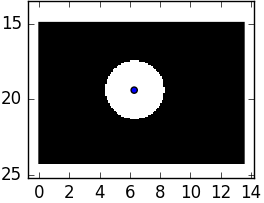
\includegraphics[scale=0.8]{python/ph2/dice_flow/ph2_MR_x100_circle@200.png}};
    \node [blockb, below of=img_t, yshift=-7cm, text width=10em] (overlap) {calculate the overlap: \\ \large \texttt{DC} = \Large $\frac{2 |A \, \cap \, B|}{|A| + |B|}$};
    % Draw edges
    \path [line] (img_t) -- (binary_t);
    \path [line] (img_t) -- (circle_t);
    \path [line] (binary) -- (overlap);
    \path [line] (circle) -- (overlap);
	\end{tikzpicture}
	\caption[Flowchart: \texttt{DC} calculation for an MR scan yielding a value of $0.9454$.]{Flowchart: \texttt{DC} calculation for an MR scan (rod \#5 @ slice 200) yielding a value of $0.9454$}
	\label{flo:DC}
\end{figure}

\subsection{Calculation: warp \& centre of mass (COM)}
\label{sec:COM}

To calculate the location shift between rods shown in CT and MRI, the coordinates of the centre of mass (COM) were subtracted.
The x- and y-shift (\texttt{warpXY}) measured in each slice was saved in an array.
Furthermore, the absolute value of the coordinate shift (\texttt{warpMagnitude}) was calculated.\\

The calculation of the \texttt{COM} is done with help of the "scipy" python package.
Its module "ndimage" contains the function "$center\_of\_mass()$", which returns the \texttt{COM}'s coordinates of a given input array.
%The values assigned to voxels in CT images lie in the range from -1024 HU (air) to around 200 HU (plastic rod).
%Before a meaningful result can be obtained, the values need to be shifted to be $>$ 0.
Only pixels representing the rod or the liquid should be used for the calculation.
Otherwise the almost black voxels surrounding the rod would influence the result.
To be regarded as part of the rod, the pixels' value has to reach a certain  \texttt{threshold}.
In order to find the relevant pixels two methods were developed:

\begin{description}
 \item[1.] a simple method calculating the number of pixels based on rod size
 \item[2.] an iteration method finding a \texttt{COM} resulting in a good \texttt{DC}
\end{description}

Both methods rely on a single reference slice to calculate the  \texttt{threshold}.
This reference should be representative for the whole scan, because the  \texttt{threshold} deduced from it will be used to find pixels belonging to the rod in all other slice, too.

\subsubsection{1. Simple Method}
The inner ($2mm$) and outer ($4mm$) radius of the plastic rods are known.
So is the pixel \texttt{spacing}, the size of a voxel in real space ($mm$).
Calculating the number of pixels which make up the more or less circular profile of the rod in a slice is calculated as follows:
\begin{align}
 pixelNumber = (radius^2 \cdot \pi) \, / \, (spacing^2)
\end{align}

For CT images the $radius = 4mm$, in MR scans the $radius = 2mm$. $spacing$ is the pixel spacing in x and y direction (developed script is only capable to process images with isotropic pixels pacing, as it usually is the case).
Next, the pixels are sorted by brightness. The top $pixelNumber$ pixels are then used to calculate the \texttt{COM}.
The value of the darkest pixel that is still counted as part of the rod is saved as  \texttt{threshold} for future calculations (e.g. finding the \texttt{DC} associated with the \texttt{COM}, see section \ref{sec:DC}).\\
The method is summarised in figure \ref{flo:COM-simple}.
Now, the DC can be obtained as described earlier using the now known \texttt{threshold} and COM coordinates.

\begin{figure}[!htb]
    \centering
	\begin{tikzpicture}[node distance = 2.5cm, auto]
    % Place nodes    
    \node [decisiony] (method) {\textbf{(1)} What image modality was used?};
    \node [blocky, left of=method, text width=11em, node distance=7cm, xshift=4cm, yshift=-3cm] (MR) {\textbf{(2a)} \large \texttt{radius = 2mm}};
    \node [blocky, right of=method, text width=11em, node distance=7cm, xshift=-4cm, yshift=-3cm] (CT) {\textbf{(2b)} \large \texttt{radius = 4mm}};
    \node [blocky, below of=method, text width=22em, yshift=-2.7cm] (pixelNumber) {\textbf{(3)} \large \texttt{pixelNumber} = \Large $\frac{radius^2 \cdot \pi}{spacing^2}$ };
    \node [blocky, below of=pixelNumber, text width=22em] (threshold) {\textbf{(4)}  Obtain value of \texttt{pixelNumber}-th brightest\\ pixel and save it as \texttt{threshold}};
    \node [blocky, below of=threshold, text width=22em] (COM) {\textbf{(5)} Use all pixels with a value above \texttt{threshold} to calculate the \texttt{COM}'s coordinates};
%    % Draw edges
    \path [line] (method.west)  to node [xshift=-1.2cm, yshift=-0.6cm] {MRI} (MR);
    \path [line] (method.east)  to node {CT} (CT);
    \path [line] (MR) -- (pixelNumber);
    \path [line] (CT) -- (pixelNumber);
    \path [line] (pixelNumber) -- (threshold);
    \path [line] (threshold) -- (COM);
	\end{tikzpicture}
	\caption[Flowchart: Simple method to find \texttt{threshold} for \texttt{COM} calculation based on real rod size.]{Flowchart: Simple method to find \texttt{threshold} for \texttt{COM} calculation based on real rod size (inner diameter: $2\,mm$, outer diameter: $4\,mm$).}
	\label{flo:COM-simple}
\end{figure}

\subsubsection{2. Iteration Method}
This algorithm is an iteration method.
Figure \ref{flo:COM-iter} shows in what order the scripts executes individual steps during the iteration.


\begin{figure}[p]
    \centering
	\begin{tikzpicture}[node distance = 3cm, auto]
    % Place nodes
    \node [blockb] (init-range) {\textbf{(1)} Start with whole range:\\\texttt{min=0\%; max=100\%}};
    \node [blockb, below of=init-range, node distance=2cm] (init-guess) {\textbf{(2)} Guess at middle of range:\\\texttt{guess =  (min+max)/2 = 50\%}};
    \node [block, below of=init-guess] (getDC) {\textbf{(3)} calculate \\\texttt{COM} coordinates and\\average \texttt{DC} for upper and\\lower half of current range:\\\texttt{DC$_{up}$ = DC @ (guess+max)/2\\ DC$_{lo}$ = DC @ (guess+min)/2}};
    \node [blockb, right of=getDC, text width=8em, node distance=6cm] (repeat!) {Repeat\\ iteration step};
    \node [decisiong, below of=getDC, node distance=3.5cm] (bigger) {\textbf{(4)} which one is bigger?};
    \node [block, left of=bigger, text width=9em, node distance=7cm, xshift=4cm, yshift=-2.5cm] (lower) {\textbf{(5a)} Neglect upper half:\\\texttt{max = guess}};
    \node [block, right of=bigger, text width=9em, node distance=7cm, xshift=-4cm, yshift=-2.5cm] (upper) {\textbf{(5b)} Neglect lower half:\\\texttt{min = guess}};
    \node [block, below of=bigger, yshift=-2.2cm] (next-guess) {\textbf{(6)} New current guess at middle of new range:\\\texttt{guess =  (min+max)/2}};
    \node [decisiong, below of=next-guess, node distance=2.5cm] (repeat) {\textbf{(7)} Repeat?};
    \node [blockb, text width=20em, below of=repeat] (fin) {\textbf{(8)} End of iteration:\\return best \texttt{DC}\\ return best \texttt{guess} (as \texttt{threshold})\\ return resulting \texttt{COM}};
    % Draw edges
    \path [line] (init-range) -- (init-guess);
    \path [line] (init-guess) -- (getDC);
    \path [line] (getDC) -- (bigger);
    \path [line] (bigger.east)  to node {\texttt{$DC_{up} > DC_{lo}$}} (upper);
    \path [line] (bigger.west)  to node [xshift=-3cm, yshift=0.8cm] {\texttt{$DC_{up} < DC_{lo}$}} (lower);
    \path [line] (lower) -- (next-guess);
    \path [line] (upper) -- (next-guess);
    \path [line] (next-guess) -- (repeat);
    \path [line] (repeat.east) -| node [xshift=-1cm, yshift=-0.5cm] {\textbf{yes}} (repeat!);
    \path [line] (repeat!) -- (getDC);
    \path [line] (repeat.south) to node {\textbf{no}} (fin);
	\end{tikzpicture}
	\caption{Flowchart: Iteration method to find \texttt{threshold}, \texttt{DC} and \texttt{COM}.}
	\label{flo:COM-iter}
\end{figure}

To begin with, it looks at the whole range of possible pixelNumbers, from $0\%$ to $100\%$ (\textbf{1}).
As a reasonable first guess it assumes that $50\%$ of all pixels belong to the rod (\textbf{2}).
Now, in the first iteration (\textbf{3}), to find out whether more or less pixels would result in a better \texttt{DC}, it considers two new guesses:
One halfway from the lower limit ($0\%$) to its current guess ($50\%$) which is:
\begin{align}
  \frac{lower + current}{2} &= \frac{0+50}{2}=25\% 
\end{align}

and one halfway from the upper limit ($100\%$) to its current guess ($50\%$) which is:
\begin{align}
 \frac{upper + current}{2} &= \frac{100+50}{2}=75\%
\end{align}


Those numbers correspond to a \texttt{threshold} each, separating the chosen percent of brighter pixels from all darker pixels in the slice.
Using the \texttt{threshold}s, the script calculates the \texttt{COM} and \texttt{DC} for both possible guesses.
%\todo{explain more}
Comparing the average over the whole rod for both \texttt{DC}s will decide which guess is closer to representing the rod better (\textbf{4}).
If the lower number of pixels yields a better average \texttt{DC} (\textbf{5a}), the upper half of the range will be neglected in the next iteration or in other words, the new upper limit takes the value of the former guess ($50\%$).
If the higher percentage yields a better average \texttt{DC} (\textbf{5b}), the lower half of the range will be neglected in the next iteration, the new lower limit takes the value of the former guess ($50\%$).
At the end of the iteration (\textbf{6}), the percentage resulting in the higher average \texttt{DC} is saved as the new current guess.
After this first iteration (\textbf{7}) the script can either repeat steps 3-6 or end it by returning the best guess and its (average) \texttt{DC} (\textbf{8}).\\

To get a better understanding, let's suppose the iteration is repeated.
At the start of the second iteration, the range is smaller (half of the entire range) and the current guess is set exactly in its middle.
If, for example, the average \texttt{DC} for $25\%$ was higher than for $75\%$, the next guess will be $25\%$, because the new range goes from $0\%$ to $50\%$.
In that case, \texttt{DC}s for the lower half of that range ($12,5\%$) and the upper half ($18,5\%$) will be calculated and compared to decide which half to eliminate in the third iteration.
If, on the other hand, the average \texttt{DC} for $75\%$ was higher, the next guess will then be $75\%$, because the new range goes from $50\%$ to $75\%$.
In that case, \texttt{DC}s for $62,5\%$ and $82,5\%$ will be compared.

The iteration continues until further steps yield no better average \texttt{DC} or a set number of steps (default setting limit is set to five iterations) has been performed.
After the iteration process, the algorithm will return the \texttt{COM} which resulted in the best DC.
The percentage of pixels that led to this \texttt{DC} is equivalent to a \texttt{threshold} which is saved for future calculations.
Figure \ref{fig:COM_iteration} shows the \texttt{DC}  found in the course of trying different percentages during the iteration method.


\begin{figure}[!thb]
\centering
  \begin{subfigure}[b]{1\textwidth}
  \centering
    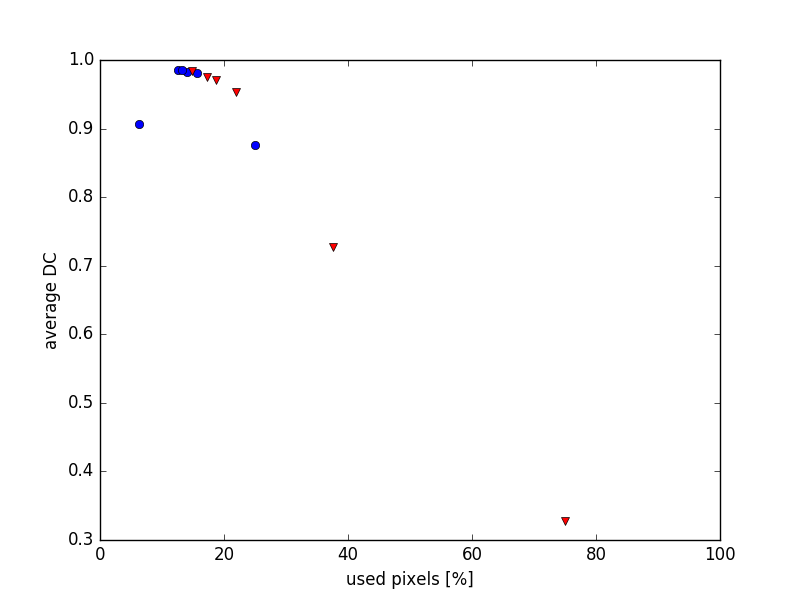
\includegraphics[scale=0.65]{python/ph3_v2/ph3_v2_CT_x100_COM_iter-far.png}
    \caption{full iteration process}
    \label{fig:CT_x100_iteration-far}
  \end{subfigure}
  \begin{subfigure}[b]{1\textwidth}
  \centering
    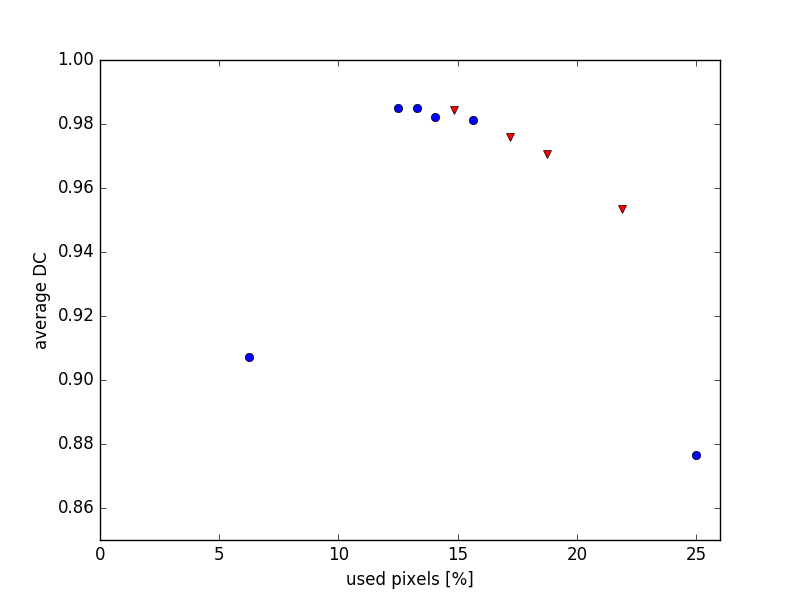
\includegraphics[scale=0.65]{python/ph3_v2/ph3_v2_CT_x100_COM_iter.png}
     \caption{close up of same iteration as in (a)}
     \label{fig:CT_x100_iteration}
  \end{subfigure}
  \caption[Example of COM iteration method, 5 repetitions.]{Example of COM iteration method, 5 repetitions, x100; red triangles correspond to upper guesses, blue dots to lower guesses.}
  \label{fig:COM_iteration}
\end{figure}


\subsection{Detection of irregularities}

The method to find irregularities is described in figure \ref{flo:irregular}.
After loading the image data, the script calculates the mean brightness of a reference slice (which was chosen by the user) (\textbf{1.}).
This reference slice will be used to decide if and which other slices might show irregularities, for example air bubbles, markers, or plastic panes.
It is the user's responsibility to make sure the reference is free from any such objects.
Ideally, it is located near the isocentre and has a brightness that is representative for the whole image.

The script will compare each slice of the volume to the reference slice individually (\textbf{2.}).
To decide whether a particular slice is "irregular", its average brightness will be compared to the reference slice's (\textbf{4.}).
If the difference exceeds a certain value (\textbf{5b.}), the current slice will be marked as irregular and consequently will not be used to calculate its \texttt{DC} or centre of mass (COM).
A value of $40\,HU$ was found to be yield good results for CT scans.


\subsubsection{Irregular slices: centre of mass \& dice coefficient}
As irregular slices cannot be used to asses distortion caused by the scanner, numbers describing their distortion are not of interest.
Instead of calculating \texttt{DC}, \texttt{COM} coordinates and warp regularly (based on the actual pixels in the slice), the values of these quantities are all set to "$-1$".
This is done, because the relevant slice was marked as not suited for distortion assessment. \\

The \texttt{COM} cannot lie outside the image, yet coordinates "($-1,-1$)" would indicate this (pixel coordinates are defined to be always positive in x and y direction).
Similarly, the value referred to as \texttt{warpMagnitude} (absolute distance between MRI and CT COM) and the \texttt{DC} are defined to be positive numbers.
All three are therefore easily understood to be invalid, indicating that the particular slice was marked as "irregular".
The values representing x- and y-shift, on the other hand, are allowed to be negative or positive.
To be consistent, they are still set to "$-1$".
It is essential to bear this in mind when interpreting the script's output.

\begin{figure}[p]
    \centering
	\begin{tikzpicture}[node distance = 3cm, auto]
    % Place nodes
    \node [blockb] (1) {\textbf{(1)} Calculate average brightness of user defined reference slice: \texttt{average(ref)}};
    \node [blockb, below of=1, node distance=2.2cm] (2) {\textbf{(2)} Initialise loop to start with slice \texttt{i=0} (first slice of Volume)};
    \node [cloud, below of=2, node distance=2.8cm] (3) {\textbf{(3)} Calculate average brightness of slice \#\texttt{i}:\\ \texttt{average(i)}};
    \node [blockb, right of=3, text width=8em, node distance=7cm] (repeat!) {Repeat comparison with next slice\\ \texttt{i $\rightarrow$ i + 1}};
    \node [decisionr, below of=3, node distance=3.5cm] (4) {\textbf{(4)} \texttt{|average(ref) - average(i)|}};
    \node [cloud, left of=4, text width=6em, node distance=7cm, xshift=3cm, yshift=-3cm] (5a) {\textbf{(5a)} mark slice \#\texttt{i} as 'regular'};
    \node [cloud, right of=4, text width=6em, node distance=7cm, xshift=-3cm, yshift=-3cm] (5b) {\textbf{(5b)} mark slice \#\texttt{i} as 'irregular'};
    \node [decisionr, below of=4, yshift=-3cm] (6) {\textbf{(6)} Has script reached\\ the last slice of the Volume?};
    \node [blockb, text width=20em, below of=6, yshift=-1cm] (7) {\textbf{(7)} End of irregularieties check};
    % Draw edges
    \path [line] (1) -- (2);
    \path [line] (2) -- (3);
    \path [line] (3) -- (4);
    \path [line] (4.east)  to node {{\texttt{> 40}}} (5b);
    \path [line] (4.west)  to node [xshift=-1.3cm, yshift=-0.5cm] {\textbf{\texttt{< 40}}} (5a);
    \path [line] (5a) -- (6);
    \path [line] (5b) -- (6);
    \path [line] (6.east) -| node [xshift=-1cm, yshift=-0.5cm] {\textbf{no}} (repeat!);
    \path [line] (repeat!) -- (3);
    \path [line] (6.south) to node {\textbf{yes}} (7);
	\end{tikzpicture}
	\caption{Flowchart: Check for irregularities.}
	\label{flo:irregular}
\end{figure}

